% Это основная команда, с которой начинается любой \LaTeX-файл. Она отвечает за тип документа, с которым связаны основные правил оформления текста.
\documentclass[12pt]{article}

% Здесь идет преамбула документа, тут пишутся команды, которые настраивают LaTeX окружение, подключаете внешние пакеты, определяете свои команды и окружения. В данном случае я это делаю в отдельных файлах, а тут подключаю эти файлы.

% Здесь я подключаю разные стилевые пакеты. Например возможности набирать особые символы или возможность компилировать русский текст. Подробное описание внутри.
\usepackage{packages}

% Здесь я определяю разные окружения, например, теоремы, определения, замечания и так далее. У этих окружений разные стили оформления, кроме того, эти окружения могут быть нумерованными или нет. Все подробно объяснено внутри.
\usepackage{environments}

% Здесь я определяю разные команды, которых нет в LaTeX, но мне нужны, например, команда \tr для обозначения следа матрицы. Или я переопределяю LaTeX команды, которые работают не так, как мне хотелось бы. Типичный пример мнимая и вещественная часть комплексного числа \Im, \Re. В оригинале они выглядят не так, как мы привыкли. Кроме того, \Im еще используется и для обозначения образа линейного отображения. Подробнее описано внутри.
\usepackage{commands}

% graphicx уже подключён в packages.sty
% Пути к рисункам указаны в \includegraphics командах напрямую

% Пакет для титульника проекта
\usepackage{titlepage}

% Здесь задаем параметры титульной страницы
% УДК для программного проекта не нужен, оставляем пустым
\setUDK{}
% Тип проекта: программный
%\setToResearch
\setToProgram

\setTitle{Прогнозирование волатильности рынка драгоценных металлов с учётом настроений инвесторов}

% Выбрать одно из трех:
% КТ1 -- \setStageOne
% КТ2 -- \setStageTwo
% Финальная версия -- \setStageFinal
%\setStageOne
%\setStageTwo
\setStageFinal

\setGroup{249}
\setStudentSgn{}
\setStudent{Лапшин Владислав Анатольевич}
\setStudentDate{}
\setAdvisor{Куренков Владимир Вячеславович}
\setAdvisorTitle{Старший преподаватель}
\setAdvisorAffiliation{Факультет компьютерных наук / Департамент больших данных и информационного поиска}
\setAdvisorDate{}
\setGrade{}
\setAdvisorSgn{}
\setYear{2026}


% С этого момента начинается текст документа
\begin{document}

% Эта команда создает титульную страницу
\makeTitlePage

% Здесь будет автоматически генерироваться содержание документа
\tableofcontents

% Аннотация — на отдельной странице (требование П1.2)
\newpage
\begin{abstract}
Работа посвящена разработке программного комплекса для прогнозирования
реализованной волатильности рынка драгоценных металлов Московской биржи
(золото GLDRUB\_TOM, серебро SLVRUB\_TOM) с учётом настроений и внимания
инвесторов. В качестве бенчмарка используется модель HAR-RV
и её расширение HAR-log-S, в которое включён лагированный
многоисточниковый sentiment-индекс (RSS, GDELT, Telegram, Google Trends).
В сравнительный анализ дополнительно включены XGBoost и kNN-поиск
исторически похожих информационных состояний на пространстве
HAR-лагов и sentiment-вектора.
Лучший результат для золота показывает HAR-log-S
($R^2_{\mathrm{OOS}} = 0{,}180$ против $0{,}177$ у бенчмарка),
для серебра~--- классическая HAR-log ($R^2_{\mathrm{OOS}} = 0{,}377$).
По тесту Диболда--Мариано улучшение от sentiment значимо
лишь на уровне 10\%; XGBoost и kNN уступают HAR-моделям на обоих инструментах.
Ablation-анализ выявил различие сильнейшего источника между активами:
для золота это взвешенный sentiment\_combined, для серебра~---
индекс внимания Google Trends. Дополнительный методологический вклад~---
единый модуль метрик с канонической Patton QLIKE и тестом Диболда--Мариано,
обеспечивающий корректное попарное сравнение моделей.
\end{abstract}

\textbf{Ключевые слова:} реализованная волатильность, HAR-RV, XGBoost, kNN,
sentiment-анализ, внимание инвесторов, Google Trends, GDELT, MOEX,
драгоценные металлы.

% \newpage по требованию П1.2 — Введение с новой страницы.
\newpage
\section*{Введение}
\addcontentsline{toc}{section}{Введение}

\subsection*{Актуальность темы исследования}
\addcontentsline{toc}{subsection}{Актуальность темы исследования}

Волатильность финансовых активов является одним из ключевых понятий в современных финансах:
она определяет стоимость опционов, влияет на управление рисками портфелей и служит
индикатором неопределённости на рынке.
Особый интерес представляет волатильность рынка драгоценных металлов~--- золота, серебра,
платины и палладия,~--- которые традиционно выступают защитными активами в периоды
геополитической нестабильности и инфляционного давления.

Начиная с 2022 года российский рынок драгоценных металлов претерпел значительные структурные
изменения: введение западных санкций, ограничение доступа к международным площадкам и
существенное изменение режима волатильности делают прогнозирование на основе
исторических закономерностей недостаточным.
В этих условиях особую ценность приобретают методы, способные учитывать
\textit{настроения инвесторов} и \textit{информационные шоки}~--- реакцию рынка на
новостной поток, изменения ключевой ставки, геополитические события.

\subsection*{Постановка проблемы}
\addcontentsline{toc}{subsection}{Постановка проблемы}

Традиционные модели прогнозирования волатильности опираются в основном на
прошлые ценовые данные и плохо учитывают информационный фон рынка. При этом
неочевидно, помогает ли добавление настроений и внимания инвесторов
прогнозировать волатильность российских драгоценных металлов и какие именно
источники полезны. Эту задачу и решает настоящая работа.

Настоящая работа посвящена разработке системы прогнозирования реализованной волатильности
(Realized Volatility, RV) инструментов Московской биржи. Программный комплекс собирает
данные по всем четырём металлам~--- GLDRUB\_TOM (золото), SLVRUB\_TOM (серебро),
PLTRUB\_TOM (платина) и PLDRUB\_TOM (палладий),~--- однако содержательный
эконометрический анализ сосредоточен на золоте и серебре: для платины и палладия
длина доступного ряда на MOEX недостаточна для надёжной оценки в режиме
расширяющегося окна (см.\ раздел~\ref{sec:results}).
В качестве бенчмарка используется классическая HAR-RV модель~\cite{Corsi2009},
которая расширяется за счёт sentiment- и attention-признаков,
извлекаемых из разнородных источников данных.

\subsection*{Цель и задачи проекта}
\addcontentsline{toc}{subsection}{Цель и задачи проекта}

\textbf{Цель работы}~--- разработать программный комплекс для
прогнозирования реализованной волатильности российских драгоценных металлов,
который объединяет эконометрические и ML-модели с многоисточниковым
вектором настроений и внимания инвесторов и предоставляет
веб-интерфейс для интерактивной визуализации прогнозов и sentiment-индексов.

\textbf{Задачи:}
\begin{enumerate}
    \item Сформировать панельный датасет дневных OHLCV-котировок драгоценных металлов
          на MOEX за период 2018--2026 гг.\ и вычислить реализованную волатильность
          оценщиком Garman--Klass (в коде также реализованы альтернативные
          оценщики Parkinson и Rogers--Satchell).
    \item Собрать многоисточниковый sentiment/attention вектор:
          новостной поток (RSS, GDELT), поисковые запросы (Google Trends),
          объёмы торгов MOEX, макроэкономические индикаторы (ЦБ РФ, FRED).
    \item Оценить HAR-RV бенчмарк и его расширения с sentiment-признаками
          методом расширяющегося окна (expanding window OOS).
    \item Реализовать и обучить модели машинного обучения на том же наборе
          признаков~--- градиентный бустинг XGBoost и kNN-прогнозировщик на
          пространстве информационных состояний (по методологии Halousková
          и Lyócsa)~--- и сравнить их с эконометрическим бенчмарком,
          в том числе по тесту Диболда--Мариано.
    \item Разработать веб-приложение для визуализации прогнозов волатильности
          и sentiment-индексов в режиме реального времени.
\end{enumerate}

\textbf{Научная новизна} работы заключается в адаптации подхода
Halousková и Lyócsa~\cite{Halouskova2025}~--- прогнозирования волатильности
через макроэкономический attention~--- к условиям российского рынка драгоценных металлов
с учётом специфики доступных источников данных (русскоязычный новостной поток,
GDELT, данные MOEX).

\textbf{Практическая значимость.}
Главная ценность работы~--- это законченный программный комплекс:
от сбора семи источников данных и расчёта волатильности до сравнения
четырёх моделей и ве2б-визуализации (более 5000 строк кода,
см.\ раздел~\ref{sec:volume}). Кроме того, в работе сделан единый модуль
метрик с QLIKE~\cite{Patton2011} и тестом Диболда--Мариано~\cite{Diebold1995}.
Видно, что добавление sentiment даёт лишь небольшой
и слабо значимый выигрыш для золота, а классическая HAR-log остаётся сильным
бенчмарком. Этот результат сам по себе полезен для риск-менеджмента.

\subsection*{Обоснование выбора инструментов и технологий}
\addcontentsline{toc}{subsection}{Обоснование выбора инструментов и технологий}

Выбор инструментов определялся задачей и доступными данными. Весь комплекс
написан на Python из-за богатой экосистемы для анализа данных и машинного
обучения (pandas, numpy, scikit-learn, xgboost). В качестве бенчмарка взята
модель HAR-RV, а не GARCH: она проста, интерпретируема и хорошо работает на
дневных данных. Для нелинейного сравнения добавлены XGBoost (стандарт для
табличных данных) и kNN на пространстве информационных состояний (по
методологии Halousková и Lyócsa). Веб-интерфейс сделан на лёгком фреймворке
Flask с интерактивными графиками Plotly. Все источники данных~--- бесплатные и
общедоступные (MOEX ISS, GDELT, Google Trends, ЦБ~РФ, FRED, RSS, Telegram),
что обеспечивает воспроизводимость результатов.


\section{Обзор литературы}

\subsection{Модели волатильности}

Исследование волатильности финансовых активов берёт начало с работ Энгла~\cite{Engle1982}
(модель ARCH) и Боллерслева~\cite{Bollerslev1986} (GARCH),
которые моделируют условную дисперсию доходностей как функцию прошлых наблюдений.
Однако GARCH-модели плохо работают на высокочастотных данных
и требуют сильных предположений о распределении остатков.

Ключевым вкладом в область прогнозирования волатильности стала модель HAR-RV
(Heterogeneous Autoregressive model of Realized Volatility), предложенная
Корси~\cite{Corsi2009}.
Модель основана на гипотезе рыночной гетерогенности: разные участники рынка
(краткосрочные трейдеры, институциональные инвесторы, пенсионные фонды) действуют
на различных временных горизонтах~--- дневном, недельном и месячном.
Спецификация HAR-RV:
\begin{equation}\label{eq:har}
    \mathrm{RV}_{t+1} = \beta_0 + \beta_d \, \mathrm{RV}_t^{(d)}
    + \beta_w \, \mathrm{RV}_t^{(w)}
    + \beta_m \, \mathrm{RV}_t^{(m)} + \varepsilon_{t+1},
\end{equation}
где $\mathrm{RV}_t^{(d)}$, $\mathrm{RV}_t^{(w)}$, $\mathrm{RV}_t^{(m)}$~---
среднеарифметические реализованные волатильности за последние 1, 5 и 22 торговых дня
соответственно.
Несмотря на линейность, модель~\eqref{eq:har} показывает хорошие
результаты на многих рынках \cite{Corsi2009}.

Для оценки качества прогнозов в работе используется QLIKE-функция
потерь~\cite{Patton2011}. Её удобство в том, что она остаётся корректной,
даже когда вместо ненаблюдаемой «истинной» волатильности подставляется
её оценка (прокси):
\begin{equation}\label{eq:qlike}
    \mathrm{QLIKE} = \mathbb{E}\!\left[
        \frac{\mathrm{RV}_t}{\hat{\sigma}_t^2}
        - \ln\!\frac{\mathrm{RV}_t}{\hat{\sigma}_t^2} - 1
    \right].
\end{equation}

\subsection{Attention и sentiment в прогнозировании}

Тетлок~\cite{Tetlock2007} одним из первых продемонстрировал, что тональность
публикаций в Wall Street Journal предсказывает доходности и объёмы торгов на фондовом рынке.
Да, Энгельберг и Гао~\cite{Da2011} предложили использовать индекс поисковой активности Google
как прямую меру внимания розничных инвесторов и показали его связь с будущими доходностями.

Работа Halousková и Lyócsa~\cite{Halouskova2025} лежит в основе настоящей работы.
Авторы строят вектор «макроэкономического внимания»~--- набор признаков,
отражающих интерес инвесторов к макроэкономическим анонсам (инфляция, ставка ФРС,
ВВП и др.)~--- и показывают, что его добавление в HAR-модель заметно улучшает
прогноз волатильности акций США.
Настоящая работа адаптирует этот подход к российскому рынку драгоценных металлов,
заменяя американские анонсы на решения ЦБ РФ, геополитические события
и данные русскоязычного новостного потока.

Для извлечения sentiment из финансовых текстов широко применяются
модели на основе BERT~\cite{Araci2019}.
FinBERT, обученный на финансовых новостях и аналитике,
работает заметно лучше словарных методов
при классификации тональности финансовых текстов.
В настоящей работе используется русскоязычная модель ruBERT
для обработки новостей российских СМИ.

\subsection{Машинное обучение для прогнозирования волатильности}

Ченом и Гестрином~\cite{Chen2016} была предложена библиотека XGBoost~---
реализация градиентного бустинга с регуляризацией,~--- ставшая стандартом
в задачах прогнозирования на табличных данных.
Применительно к финансовым временным рядам XGBoost позволяет нелинейно
комбинировать HAR-признаки с sentiment-вектором без явного задания функциональной формы.

Рекуррентные нейронные сети, в частности LSTM~\cite{Hochreiter1997},
способны улавливать долгосрочные зависимости в последовательностях,
что делает их естественным выбором для моделирования волатильности
с явной последовательной структурой.

\subsection{Волатильность рынка драгоценных металлов}

Рынок драгоценных металлов характеризуется рядом особенностей,
отличающих его от рынков акций:
высокой чувствительностью к геополитическим событиям и инфляционным ожиданиям,
ролью золота как «safe haven» актива и значительным влиянием
курса доллара США на рублёвые цены инструментов MOEX.
Российский рынок металлов после 2022 года приобрёл дополнительную специфику
в связи с ограничениями на экспорт и реструктуризацией торговых потоков,
что создаёт нетривиальные задачи для прогнозирования.

\section{Описание функциональных и нефункциональных требований}
\label{sec:requirements}

\subsection{Общее описание системы}

Разрабатываемый программный комплекс представляет собой модульную систему
для сбора данных, обучения моделей прогнозирования волатильности
и визуализации результатов.
Система реализована на языке Python~3.11+ и состоит из четырёх подсистем:
сбора данных, обработки и агрегации признаков, модельного модуля и веб-интерфейса.

\subsection{Функциональные требования}

\textbf{Подсистема сбора данных} обязана:
\begin{enumerate}
    \item Загружать дневные OHLCV-котировки инструментов GLDRUB\_TOM, SLVRUB\_TOM,
          PLTRUB\_TOM, PLDRUB\_TOM с MOEX ISS API за произвольный исторический период.
    \item Парсить новостные RSS-ленты российских финансовых СМИ
          (Коммерсантъ, Ведомости, Интерфакс, ТАСС, РБК, Investing.com)
          с фильтрацией по ключевым словам, связанным с металлами и макроэкономикой.
    \item Загружать данные GDELT Global Knowledge Graph за заданный период
          и извлекать дневные агрегаты тональности (Tone) и количества статей.
    \item Получать индексы поисковой активности Google Trends
          по релевантным запросам через библиотеку \texttt{pytrends}.
    \item Загружать официальные курсы валют (USD/RUB, EUR/RUB, CNY/RUB)
          и историю ключевой ставки с XML API Банка России.
    \item Загружать макроэкономические ряды (нефть Brent, VIX, DXY, CPI США)
          через FRED API.
    \item Все источники данных должны поддерживать инкрементальное обновление:
          повторный запуск не перезаписывает существующие данные.
\end{enumerate}

\textbf{Подсистема обработки признаков} обязана:
\begin{enumerate}
    \item Вычислять дневную реализованную волатильность из OHLCV-данных
          методами Garman--Klass, Parkinson, Rogers--Satchell и Close-to-Close.
    \item Формировать HAR-лаги ($\mathrm{RV}^{(d)}$, $\mathrm{RV}^{(w)}$, $\mathrm{RV}^{(m)}$)
          для каждого инструмента.
    \item Агрегировать все источники sentiment и attention
          в единый дневной CSV-файл с полным временным покрытием.
\end{enumerate}

\textbf{Модельный модуль} обязан:
\begin{enumerate}
    \item Реализовывать HAR-RV модель в трёх спецификациях:
          уровни (HAR-level), логарифмы (HAR-log) и
          логарифмы с sentiment (HAR-log-S).
    \item Проводить оценку методом расширяющегося окна (expanding window)
          с метриками MAE, RMSE, QLIKE и $R^2_{\mathrm{OOS}}$.
    \item Реализовывать модели машинного обучения на тех же наборах
          признаков: градиентный бустинг XGBoost и kNN-прогнозировщик
          на пространстве информационных состояний.
    \item Сохранять результаты прогнозов и метрики в CSV для последующего анализа.
\end{enumerate}

\textbf{Веб-интерфейс} обязан:
\begin{enumerate}
    \item Отображать исторический график реализованной волатильности
          с наложением прогнозов модели.
    \item Отображать дашборд sentiment-индексов по источникам.
    \item Обновляться при запуске скрипта обновления данных.
\end{enumerate}

\subsection{Нефункциональные требования}

\begin{enumerate}
    \item \textbf{Воспроизводимость.}
          Все случайные процессы фиксируются через \texttt{random\_state=42}.
          Зависимости фиксируются в \texttt{requirements.txt}.
    \item \textbf{Модульность.}
          Каждый источник данных реализован в отдельном модуле
          с единым интерфейсом командной строки.
    \item \textbf{Расширяемость.}
          Добавление нового источника данных не требует изменения модельного модуля.
    \item \textbf{Производительность.}
          Полный цикл обновления данных и переобучения моделей должен завершаться
          не более чем за 30 минут на стандартном ноутбуке.
    \item \textbf{Открытость данных.}
          Все используемые источники данных должны быть бесплатно доступны
          без ограничений на некоммерческое использование.
\end{enumerate}

\section{Сравнение с существующими аналогами}

Разработанная система прогнозирует волатильность с помощью альтернативных
источников данных. Ниже рассмотрены наиболее близкие аналоги~---
коммерческие платформы, открытые библиотеки и академические системы.

\subsection{Коммерческие платформы}

\textbf{Bloomberg Terminal / Refinitiv Eikon.}
Профессиональные терминалы предоставляют широкий набор инструментов
для анализа волатильности: реализованную волатильность, подразумеваемую волатильность,
исторические ряды VIX-подобных индексов.
Тем не менее эти платформы ориентированы на западные рынки,
не имеют готовых sentiment-моделей для русскоязычного контента,
а доступ к данным по инструментам MOEX после 2022~г.\ существенно ограничен.
Стоимость подписки ($>$\$20\,000 в год) исключает использование в академических проектах.

\textbf{MOEX Analytics.}
Официальный аналитический портал Московской биржи предоставляет
исторические данные OHLCV и простые индикаторы волатильности
(скользящее стандартное отклонение).
Инструменты машинного обучения, альтернативные источники данных
и функционал прогнозирования в платформе отсутствуют.

\subsection{Открытые библиотеки}

\textbf{arch (Python).}
Библиотека~\texttt{arch}~\cite{Sheppard2017} реализует широкий спектр
GARCH-семейства моделей (GARCH, EGARCH, GJR-GARCH и др.)
и является стандартом для параметрического моделирования волатильности.
Однако библиотека не поддерживает HAR-RV модели, не имеет встроенного
сбора данных и не работает с альтернативными источниками.
Настоящая система использует HAR-RV как бенчмарк,
а не GARCH, что обусловлено недоступностью высокочастотных данных.

\textbf{FinRL (AI4Finance).}
Фреймворк для обучения с подкреплением в финансах~\cite{Liu2021}
предоставляет среды для торговли акциями с базовыми техническими признаками.
FinRL не ориентирован на задачу прогнозирования волатильности,
не поддерживает sentiment-признаки из внешних API
и не имеет модулей для работы с MOEX.

\textbf{Qlib (Microsoft).}
Исследовательская платформа для количественных финансов~\cite{Yang2020}
включает обширный набор ML-моделей для прогнозирования доходностей.
Поддержка данных ограничена американскими и китайскими рынками;
модуль прогнозирования волатильности отсутствует;
русскоязычный sentiment не поддерживается.

\subsection{Академические системы}

В работе~\cite{Halouskova2025} предложена система прогнозирования
волатильности акций США на основе вектора макроэкономического внимания.
Настоящий проект является адаптацией этой методологии
для российского рынка драгоценных металлов:
заменены источники внимания (американские макроанонсы~→
решения ЦБ РФ, русскоязычные Telegram-каналы, GDELT-тональность)
и рыночные данные (S\&P~500~→ MOEX GLDRUB\_TOM / SLVRUB\_TOM).

\subsection{Сводная таблица сравнения}

\begin{table}[H]
\centering
\caption{Сравнение разработанной системы с аналогами}
\label{tab:analogs}
\small
\begin{tabular}{p{3.4cm}ccccc}
\hline
Характеристика
  & \rotatebox{70}{Bloomberg}
  & \rotatebox{70}{arch}
  & \rotatebox{70}{FinRL}
  & \rotatebox{70}{Qlib}
  & \rotatebox{70}{\textbf{Наша система}} \\
\hline
Данные MOEX              & $\pm$ & ---  & --- & --- & \textbf{+} \\
HAR-RV модель            & ---   & ---  & --- & --- & \textbf{+} \\
XGBoost / kNN            & ---   & ---  & +   & +   & \textbf{+} \\
Русскоязычный sentiment  & ---   & ---  & --- & --- & \textbf{+} \\
Telegram-парсер          & ---   & ---  & --- & --- & \textbf{+} \\
GDELT-тональность        & $\pm$ & ---  & --- & --- & \textbf{+} \\
Google Trends attention  & ---   & ---  & --- & --- & \textbf{+} \\
Макро ЦБ РФ              & ---   & ---  & --- & --- & \textbf{+} \\
Инкрементальное обновление& +    & ---  & --- & +   & \textbf{+} \\
Веб-интерфейс            & +     & ---  & --- & $\pm$ & \textbf{+} \\
Открытый исходный код    & ---   & +    & +   & +   & \textbf{+} \\
Бесплатный доступ        & ---   & +    & +   & +   & \textbf{+} \\
\hline
\end{tabular}

\medskip
\raggedright
\footnotesize
\textit{Обозначения:} «+»~--- поддерживается; «---»~--- отсутствует;
«$\pm$»~--- частичная поддержка.
\end{table}

Видно, что среди рассмотренных решений нет ни одного, которое
одновременно работает с данными MOEX, русскоязычным sentiment
и моделями прогнозирования волатильности (HAR-RV, бустинг, kNN).
Именно это сочетание и отличает разработанную систему от существующих
аналогов для российского рынка драгоценных металлов.

\section{Архитектура программного комплекса}

\subsection{Общая структура}

Программный комплекс реализован на языке Python~3.11 и организован
по принципу конвейера данных (data pipeline):
независимые модули сбора данных формируют единый входной датасет,
который передаётся в модельный модуль, а результаты прогноза
отображаются через веб-интерфейс.
Архитектура системы представлена на рисунке~\ref{fig:architecture}.

\begin{figure}[H]
\centering
\resizebox{\linewidth}{!}{%
\begin{tikzpicture}[
    font=\small,
    %% стили узлов
    source/.style = {draw, rounded corners=3pt, fill=blue!10,
                     minimum width=3.0cm, minimum height=0.65cm,
                     align=center, text width=2.9cm},
    parser/.style = {draw, rounded corners=3pt, fill=orange!18,
                     minimum width=3.4cm, minimum height=0.65cm,
                     align=center, text width=3.3cm},
    store/.style  = {draw, rounded corners=3pt, fill=yellow!25,
                     minimum width=3.2cm, minimum height=0.65cm,
                     align=center, text width=3.1cm,
                     font=\small\ttfamily},
    proc/.style   = {draw, rounded corners=3pt, fill=green!14,
                     minimum width=3.6cm, minimum height=0.65cm,
                     align=center, text width=3.5cm},
    dsfile/.style = {draw, rounded corners=3pt, fill=yellow!30,
                     minimum width=3.4cm, minimum height=0.65cm,
                     align=center, text width=3.3cm,
                     font=\small\ttfamily},
    model/.style  = {draw, rounded corners=3pt, fill=violet!14,
                     minimum width=3.6cm, minimum height=0.65cm,
                     align=center, text width=3.5cm},
    outstyle/.style = {draw, rounded corners=3pt, fill=red!10,
                     minimum width=3.4cm, minimum height=0.65cm,
                     align=center, text width=3.3cm},
    hdr/.style    = {font=\small\itshape, text=gray!70},
    arr/.style    = {-{Stealth[length=5pt,width=4pt]}, semithick},
]

%% ═══════════════════════════════════════════════════════
%% Шаг по оси Y между строками
\def\dy{1.25}

%% ═══════════════════════════════════════════════════════
%% Колонка 1 — Источники  (x=0)
\foreach \lbl/\n in {
    {MOEX ISS API}/0,
    {RSS-ленты (6)}/1,
    {GDELT GKG}/2,
    {Telegram API}/3,
    {Google Trends}/4,
    {ЦБ РФ XML API}/5,
    {FRED API}/6}
  \node[source] (src\n) at (0, -\n*\dy) {\lbl};

%% ═══════════════════════════════════════════════════════
%% Колонка 2 — Парсеры  (x=4.5)
\foreach \lbl/\n in {
    {download\_moex.py}/0,
    {parse\_rss.py}/1,
    {parse\_gdelt.py}/2,
    {parse\_telegram.py}/3,
    {parse\_google\_trends.py}/4,
    {parse\_cbr.py}/5,
    {parse\_fred.py}/6}
  \node[parser] (par\n) at (4.5, -\n*\dy) {\lbl};

%% стрелки col1 → col2
\foreach \n in {0,1,2,3,4,5,6}
  \draw[arr] (src\n) -- (par\n);

%% ═══════════════════════════════════════════════════════
%% Колонка 3 — CSV-файлы  (x=9.5)
\foreach \lbl/\n in {
    {OHLCV\_1d.csv}/0,
    {rss\_news.csv}/1,
    {gdelt\_sent.csv}/2,
    {telegram\_sent.csv}/3,
    {google\_trends.csv}/4,
    {cbr\_data.csv}/5,
    {fred\_macro.csv}/6}
  \node[store] (csv\n) at (9.5, -\n*\dy) {\lbl};

%% стрелки col2 → col3
\foreach \n in {0,1,2,3,4,5,6}
  \draw[arr] (par\n) -- (csv\n);

%% ═══════════════════════════════════════════════════════
%% Колонка 4 — Обработка  (x=14.5)
%% compute_rv.py  принимает только csv0 (OHLCV)
%% aggregate_sentiment.py принимает csv1..csv6

\node[proc]   (rv)   at (14.5, -0.5*\dy) {compute\_rv.py};
\node[dsfile] (dsrv) at (14.5, -2.0*\dy) {rv\_features.csv};
\node[proc]   (agg)  at (14.5, -3.5*\dy) {aggregate\_sentiment.py};
\node[dsfile] (dsst) at (14.5, -5.0*\dy) {daily\_sentiment.csv};

%% OHLCV → compute_rv → rv_features.csv
\draw[arr] (csv0.east) -- ++(0.35,0) |- (rv.west);
\draw[arr] (rv.south)  -- (dsrv.north);

%% csv1..csv6 → aggregate → daily_sentiment
\foreach \n in {1,2,3,4,5,6}
  \draw[arr] (csv\n.east) -- ++(0.35,0) |- (agg.west);
\draw[arr] (agg.south) -- (dsst.north);

%% ═══════════════════════════════════════════════════════
%% Колонка 5 — Модели  (x=19.5)

\node[model] (har)  at (19.5, -0.5*\dy)  {har\_model.py\\\footnotesize(HAR-log / HAR-log-S)};
\node[model] (xgb)  at (19.5, -2.5*\dy)  {ml\_models.py\\\footnotesize(XGBoost)};
\node[model] (lstm) at (19.5, -4.5*\dy)  {knn\_model.py\\\footnotesize(kNN)};

%% rv_features → модели
\draw[arr] (dsrv.east) -- ++(0.35,0) |- (har.west);
\draw[arr] (dsrv.east) -- ++(0.35,0) |- (xgb.west);
\draw[arr] (dsrv.east) -- ++(0.35,0) |- (lstm.west);

%% daily_sentiment → XGBoost, LSTM
\draw[arr] (dsst.east) -- ++(0.35,0) |- (xgb.west);
\draw[arr] (dsst.east) -- ++(0.35,0) |- (lstm.west);

%% ═══════════════════════════════════════════════════════
%% Колонка 6 — Вывод  (x=24.5)

\node[outstyle] (res) at (24.5, -2.5*\dy) {ml\_results/*.csv};
\node[outstyle] (web) at (24.5, -5.0*\dy) {Flask app.py\\\footnotesize(веб-интерфейс)};

%% модели → результаты
\foreach \m in {har,xgb,lstm}
  \draw[arr] (\m.east) -- ++(0.35,0) |- (res.west);

%% результаты → веб
\draw[arr] (res.south) -- (web.north);

%% daily_sentiment → веб (данные для дашборда)
\draw[arr] (dsst.east) -- ++(5.85,0) |- (web.west);

%% ═══════════════════════════════════════════════════════
%% Заголовки колонок
\node[hdr] at (0,    0.75) {Источники};
\node[hdr] at (4.5,  0.75) {Парсеры};
\node[hdr] at (9.5,  0.75) {CSV-файлы};
\node[hdr] at (14.5, 0.75) {Обработка};
\node[hdr] at (19.5, 0.75) {Модели};
\node[hdr] at (24.5, 0.75) {Вывод};

\end{tikzpicture}%
}%
\caption{Архитектура программного комплекса прогнозирования волатильности.
         Стрелки~--- направление потока данных.}
\label{fig:architecture}
\end{figure}

\subsection{Подсистема сбора данных}

Каждый источник данных инкапсулирован в отдельном модуле
в директории \texttt{src/data/}.
Все парсеры поддерживают инкрементальное обновление:
при повторном запуске новые данные дописываются к существующему файлу
без перезаписи исторических наблюдений.
Интерфейс командной строки унифицирован: параметры \texttt{-{}-from}
и \texttt{-{}-to} задают временной диапазон выгрузки.

\textbf{download\_moex.py} --- загружает дневные OHLCV-котировки
инструментов GLDRUB\_TOM, SLVRUB\_TOM, PLTRUB\_TOM, PLDRUB\_TOM
через MOEX ISS REST API (формат JSON, пагинация по 100 записей).
Выходной файл: \texttt{data/raw/<SECID>\_1d.csv}.

\textbf{parse\_rss.py} --- парсит RSS-ленты шести финансовых изданий
(Коммерсантъ, Ведомости, Интерфакс, ТАСС, РБК, Investing.com)
с фильтрацией по 54 ключевым словам.
Сентимент статей вычисляется моделью ruBERT (HuggingFace) для каждой статьи
и агрегируется в дневной score.

\textbf{parse\_gdelt.py} --- загружает суточные CSV-архивы
GDELT Global Knowledge Graph (GKG v2) за указанный период
и извлекает усреднённый индекс тональности Tone по тематическим кластерам,
связанным с золотом, серебром и российской экономикой.

\textbf{parse\_telegram.py} --- использует Telethon MTProto API
для чтения 12 публичных русскоязычных каналов финансовой тематики
(\textit{@russianmacro}, \textit{@bcs\_express}, \textit{@cbrstocks},
\textit{@markettwits} и др.).
Тексты фильтруются по 36 ключевым словам; лексический scorer
взвешивает позитивные и негативные упоминания по числу просмотров сообщения.

\textbf{parse\_google\_trends.py} --- загружает недельные индексы
поисковой активности через \texttt{pytrends} по трём группам запросов
(metals\_ru, macro\_ru, metals\_en) и интерполирует до дневной частоты.

\textbf{parse\_cbr.py} --- обращается к XML API Банка России
для получения официальных курсов валют (USD/RUB, EUR/RUB, CNY/RUB)
и истории ключевой ставки.

\textbf{parse\_fred.py} --- загружает макроэкономические ряды
через FRED API: нефть Brent (DCOILBRENTEU), индекс доллара США (DTWEXBGS),
волатильность VIX (VIXCLS), ставку ФРС (FEDFUNDS), CPI США (CPIAUCSL).

\subsection{Подсистема обработки признаков}

\textbf{compute\_rv.py} принимает OHLCV-данные и вычисляет
дневную реализованную волатильность четырьмя методами
(Garman--Klass, Parkinson, Rogers--Satchell, Close-to-Close),
формирует HAR-лаги $\mathrm{RV}^{(d)}, \mathrm{RV}^{(w)}, \mathrm{RV}^{(m)}$
и сохраняет результат в \texttt{data/processed/rv\_features.csv}.

\textbf{aggregate\_sentiment.py} объединяет выходные файлы всех семи
парсеров в единый датафрейм с дневной частотой.
При слиянии применяется:
\textit{forward fill} для числовых рядов (курсы, макроэкономика),
\textit{заполнение нулями} для sentiment-переменных в дни без новостей,
\textit{z-score нормализация} с скользящим окном 30 дней
для объёмов торгов и их sigmoid-преобразование.
Итоговый файл \texttt{daily\_sentiment.csv} содержит 25 признаков.

Комбинированный sentiment-индекс вычисляется как взвешенная сумма:
\begin{equation}\label{eq:sent_comb}
    S_t^{\text{comb}} = 0{,}4 \cdot S_t^{\text{RSS}}
                      + 0{,}4 \cdot S_t^{\text{GDELT}}
                      + 0{,}2 \cdot S_t^{\text{Telegram}},
\end{equation}
где веса отражают качество покрытия: RSS и GDELT имеют более полное
временное охватывание, чем Telegram-архив.

\subsection{Модельный модуль}

Модельный модуль разделён на два файла.

\textbf{har\_model.py} реализует эконометрический пайплайн:
формирование HAR-матрицы дизайна, оценку МНК с поправкой HAC
(библиотека \texttt{statsmodels}), процедуру расширяющегося окна
и расчёт метрик.

\textbf{ml\_models.py} реализует основную модель XGBoost
на расширенном наборе HAR-лагов и sentiment/attention-признаков
с лагом~1 относительно целевой переменной.
Используется библиотека \texttt{xgboost}; гиперпараметры приведены
в разделе с описанием методологии.
В модуле также реализован LSTM, но в итоговое сравнение он не вошёл:
на дневной выборке такой длины его результаты оказались нестабильными.
Все модельные классы (\texttt{HARModel}, \texttt{XGBoostRV}, \texttt{LSTMRVModel})
имеют единый интерфейс \texttt{fit(X, y)}, \texttt{predict(X)},
\texttt{evaluate(X, y) → dict}, что позволяет легко добавлять новые
модели в общий пайплайн оценивания.
Единая для всех моделей реализация метрик (MAE, RMSE,
$R^2_{\mathrm{OOS}}$, QLIKE) и тест Диболда--Мариано вынесены
в модуль \texttt{src/models/metrics.py}.

Структура ключевых классов модельного модуля приведена
в таблице~\ref{tab:classes}.

\begin{table}[h!]
\centering
\caption{Ключевые классы и функции модельного модуля}
\label{tab:classes}
\small
\begin{tabular}{p{3.4cm}p{4.0cm}p{6.5cm}}
\hline
Класс / функция & Модуль & Назначение и ключевые методы \\
\hline
\texttt{HARModel}
  & \texttt{models/har\_model.py}
  & Эконометрическая HAR-RV модель.
    Атрибуты: \texttt{spec} (level/log/log\_sentiment),
    \texttt{sentiment\_col}, \texttt{train\_frac}.
    Методы: \texttt{fit\_rolling()},
    \texttt{fit\_full()},
    \texttt{metrics()},
    \texttt{save\_results()}. \\
\texttt{XGBoostRV}
  & \texttt{models/ml\_models.py}
  & Градиентный бустинг XGBoost
    на расширенном наборе признаков.
    Методы: \texttt{fit(X, y)},
    \texttt{predict(X)},
    \texttt{evaluate(X, y)},
    \texttt{feature\_importance()}. \\
\texttt{LSTMRVModel}
  & \texttt{models/ml\_models.py}
  & Рекуррентная сеть (PyTorch) с early stopping;
    не используется в финальном сравнении из-за
    нестабильности на дневной выборке. \\
\texttt{run\_knn(...)}
  & \texttt{models/knn\_model.py}
  & Expanding-window kNN на пространстве
    HAR$+$sentiment с inverse-distance ядром
    и подобранными $k^*=75/30$. \\
\texttt{compute\_metrics(...)}
  & \texttt{models/metrics.py}
  & Единый расчёт MAE, RMSE, $R^2_{\mathrm{OOS}}$
    и Patton QLIKE (с авто-\texttt{exp()} для log-моделей). \\
\texttt{diebold\_mariano(...)}
  & \texttt{models/metrics.py}
  & DM-тест с HAC-стандартной ошибкой
    (Newey--West, ядро Бартлетта). \\
\hline
\end{tabular}
\end{table}

\subsection{Веб-интерфейс}

Веб-интерфейс реализован на микрофреймворке Flask и запускается
локально командой \texttt{python3 app.py}.
При открытии страницы \texttt{http://localhost:5000} пользователю
доступны три страницы:

\begin{enumerate}
    \item \textbf{Обзор} (\texttt{/})~--- временные ряды реализованной
          волатильности золота и серебра и сводная таблица метрик моделей.
    \item \textbf{Прогноз волатильности} (\texttt{/volatility})~---
          интерактивный временной ряд реализованной волатильности
          с наложением прогноза модели за последние месяцы.
    \item \textbf{Sentiment-монитор} (\texttt{/sentiment})~---
          панели с динамикой комбинированного sentiment-индекса,
          Telegram-score, индекса внимания Google Trends и
          макроэкономических индикаторов.
\end{enumerate}

Данные загружаются из CSV-файлов при каждом обращении к странице,
что обеспечивает автоматическое обновление визуализации после
запуска скриптов обновления данных.
Стек: Flask~3.0, Plotly~5 (интерактивные графики), Bootstrap~5 (вёрстка).

\subsection{Демонстрация системы с точки зрения пользователя}
\label{sec:demo}

С точки зрения конечного пользователя (аналитика или риск-менеджера)
типовой сценарий работы с комплексом выглядит так: пользователь запускает
\texttt{python3 app.py}, открывает страницу обзора и оценивает текущий
уровень и динамику реализованной волатильности по золоту и серебру; затем
переходит на страницу прогноза, где визуально сопоставляет фактическую
волатильность с прогнозом модели (рисунок~\ref{fig:ui_forecast}), и на
sentiment-монитор, чтобы соотнести всплески волатильности с изменением
информационного фона. Вся навигация осуществляется без перезагрузки данных
вручную и без знания внутренней структуры проекта.

На странице прогноза для каждого инструмента строится график логарифма
реализованной волатильности: сплошной линией~--- факт, пунктиром~--- прогноз
XGBoost на тестовой выборке (последние 40\% наблюдений). По нему видно, что
модель в целом повторяет уровень волатильности, но сглаживает резкие
всплески~--- это совпадает с числовыми результатами раздела~\ref{sec:results}.

\begin{figure}[H]
\centering
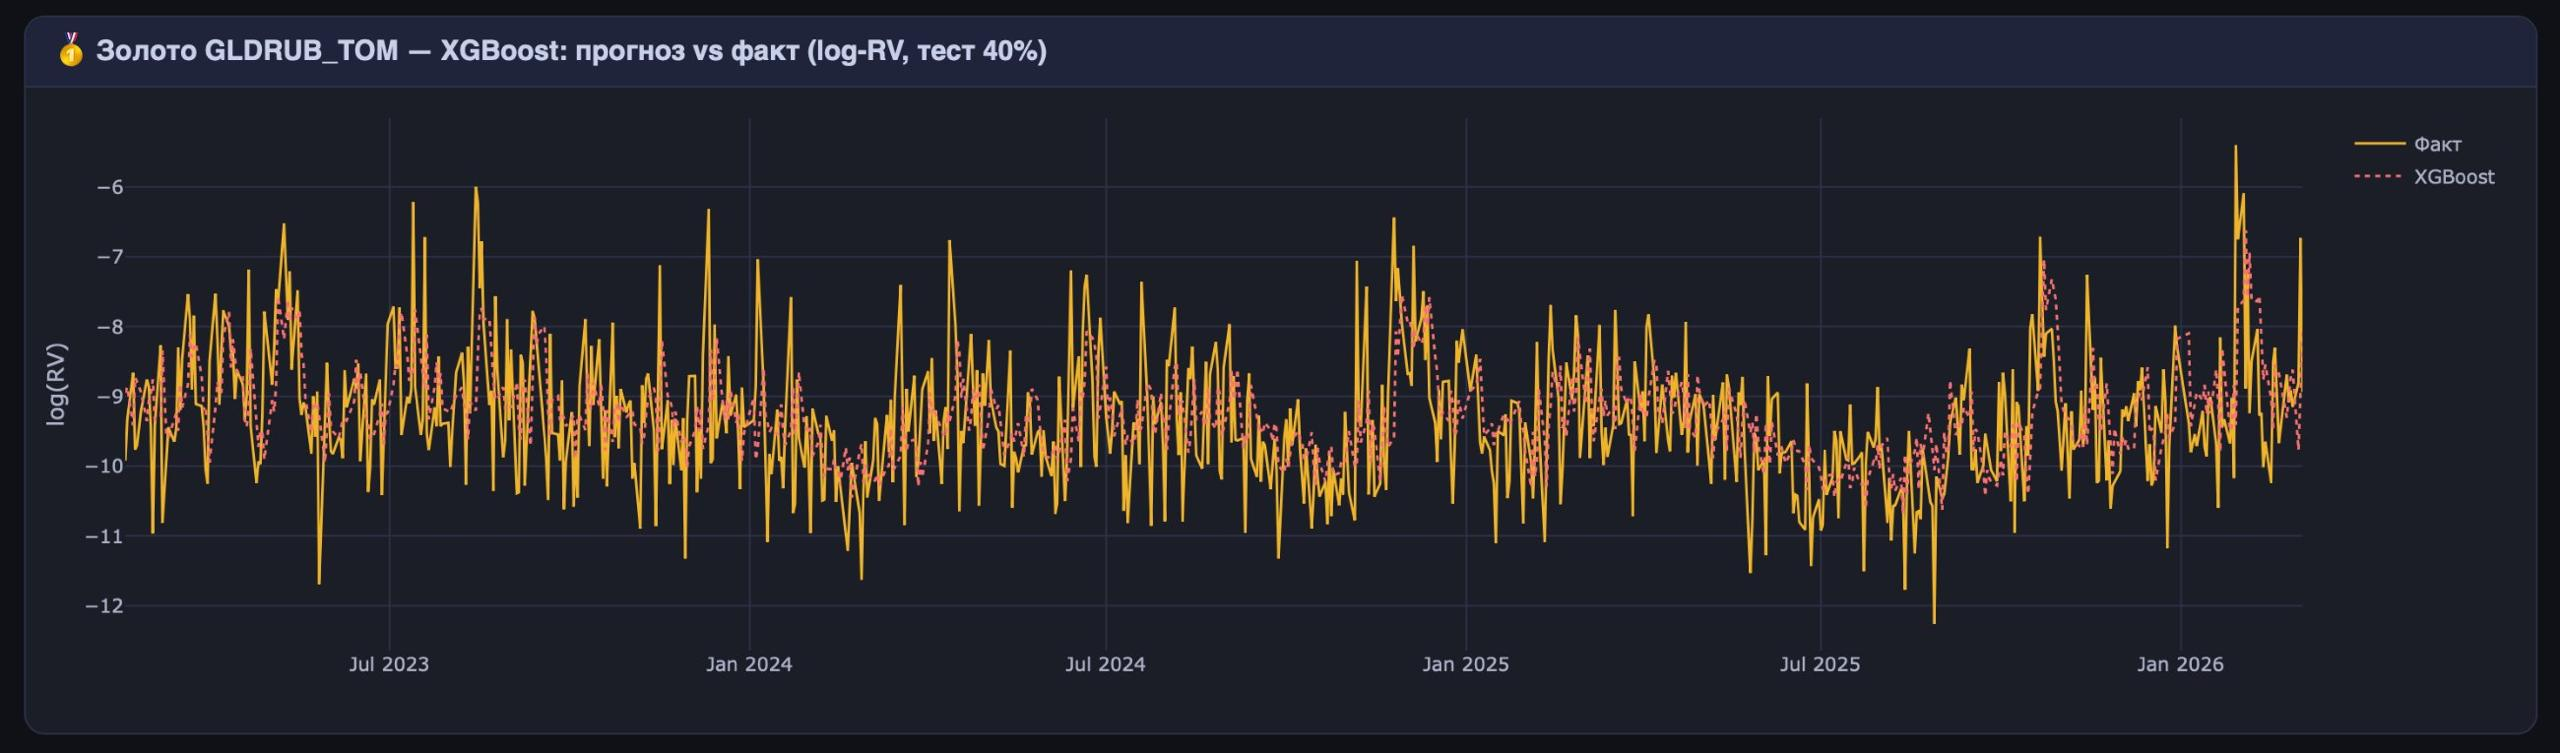
\includegraphics[width=\linewidth]{figures/ui_forecast_gld.png}\\[4pt]
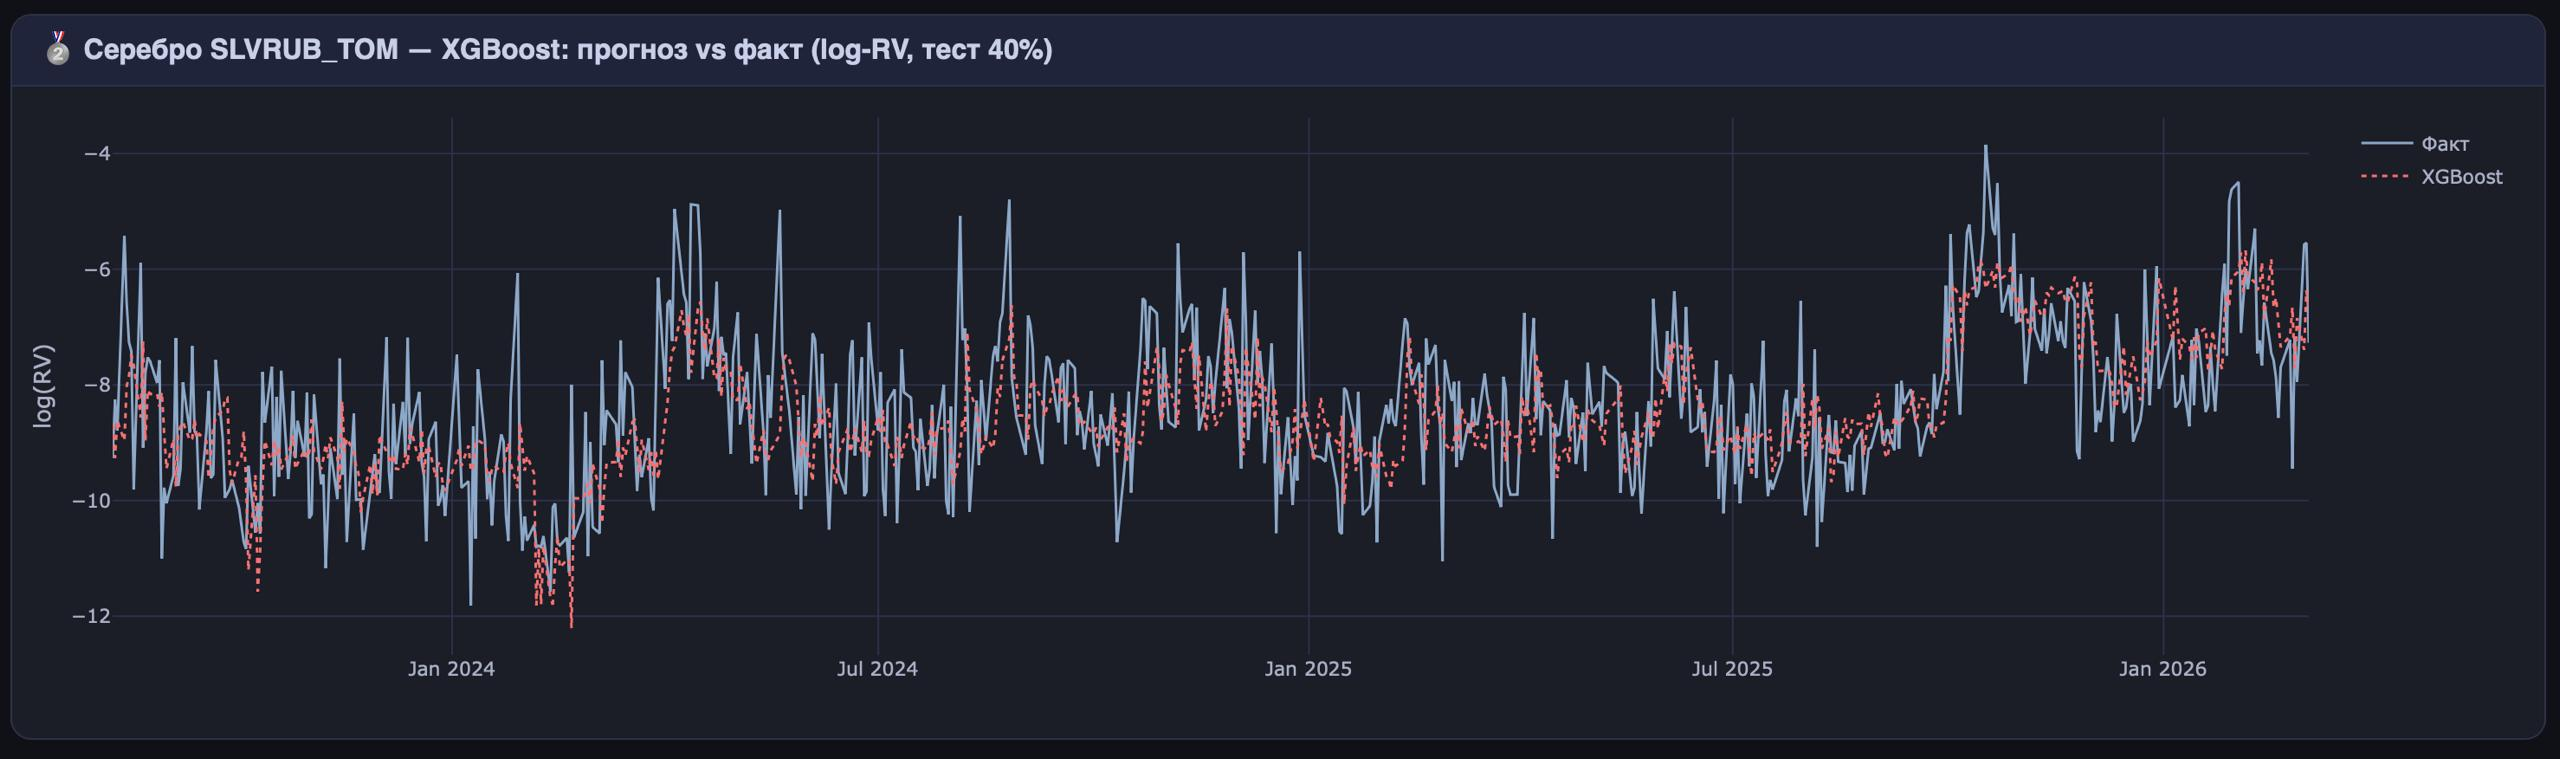
\includegraphics[width=\linewidth]{figures/ui_forecast_slv.png}
\caption{Страница прогноза веб-интерфейса: сопоставление фактической
реализованной волатильности (log-RV) с прогнозом XGBoost на тестовой
выборке для золота (GLDRUB\_TOM, сверху) и серебра (SLVRUB\_TOM, снизу).}
\label{fig:ui_forecast}
\end{figure}

\section{Данные}

\subsection{Котировки драгоценных металлов}

Основным источником рыночных данных служит MOEX ISS API~---
открытый интерфейс Московской биржи.
Загружаются дневные OHLCV-данные (цены открытия, максимума, минимума, закрытия
и объём торгов) для четырёх инструментов:

\begin{itemize}
    \item \textbf{GLDRUB\_TOM}~--- золото в рублях, данные с 9 января 2018 г.,
          2\,031 торговый день;
    \item \textbf{SLVRUB\_TOM}~--- серебро в рублях, данные с 9 января 2018 г.,
          1\,926 торговых дней;
    \item \textbf{PLTRUB\_TOM}~--- платина в рублях, данные с 22 октября 2024 г.,
          346 торговых дней;
    \item \textbf{PLDRUB\_TOM}~--- палладий в рублях, данные с 22 октября 2024 г.,
          346 торговых дней.
\end{itemize}

Ввиду ограниченности исторических данных по платине и палладию
основной акцент в эмпирическом анализе делается на золоте и серебре.

\subsection{Реализованная волатильность}

Поскольку внутридневные тиковые данные недоступны, реализованная
волатильность считается по дневным OHLC-ценам с помощью range-based
оценщиков~\cite{Garman1980, Parkinson1980}. Они точнее обычного
оценщика по ценам закрытия (Close-to-Close), так как используют ещё
максимум и минимум дня.

\textbf{Оценщик Garman--Klass}~\cite{Garman1980} (используется как основной):
\begin{equation}\label{eq:gk}
    \widehat{\sigma}^2_t = \tfrac{1}{2}\bigl(\ln H_t - \ln L_t\bigr)^2
    - \bigl(2\ln 2 - 1\bigr)\bigl(\ln C_t - \ln O_t\bigr)^2,
\end{equation}
где $O_t, H_t, L_t, C_t$~--- цены открытия, максимума, минимума и закрытия в день $t$.
Эффективность оценщика~\eqref{eq:gk} примерно в 7{,}4 раза выше, чем у Close-to-Close.

\textbf{Оценщик Parkinson}~\cite{Parkinson1980}:
\begin{equation}\label{eq:park}
    \widehat{\sigma}^2_t = \frac{\bigl(\ln H_t - \ln L_t\bigr)^2}{4 \ln 2}.
\end{equation}

Аннуализированная волатильность вычисляется как
$\widehat{\sigma}^{\mathrm{ann}}_t = \sqrt{252 \cdot \widehat{\sigma}^2_t}$.
Описательные статистики для основных инструментов приведены в таблице~\ref{tab:rv_stats}.

\begin{table}[h!]
\centering
\caption{Описательные статистики аннуализированной волатильности (оценщик Garman--Klass)}
\label{tab:rv_stats}
\begin{tabular}{lrrrrrr}
\hline
Инструмент & $N$ & Среднее & Медиана & Станд.\ откл. & Минимум & Максимум \\
\hline
GLDRUB\_TOM & 1\,931 & 0{,}156 & 0{,}115 & 0{,}166 & 0{,}001 & 1{,}659 \\
SLVRUB\_TOM & 1\,635 & 0{,}276 & 0{,}196 & 0{,}270 & 0{,}001 & 2{,}317 \\
\hline
\end{tabular}
\end{table}

На рисунке~\ref{fig:rv_timeseries} представлена динамика аннуализированной
реализованной волатильности обоих инструментов за весь период наблюдений.
Вертикальная пунктирная линия отмечает 24 февраля 2022~г.~---
момент резкого скачка волатильности, образующего структурный разрыв в ряду.

\begin{figure}[H]
\centering
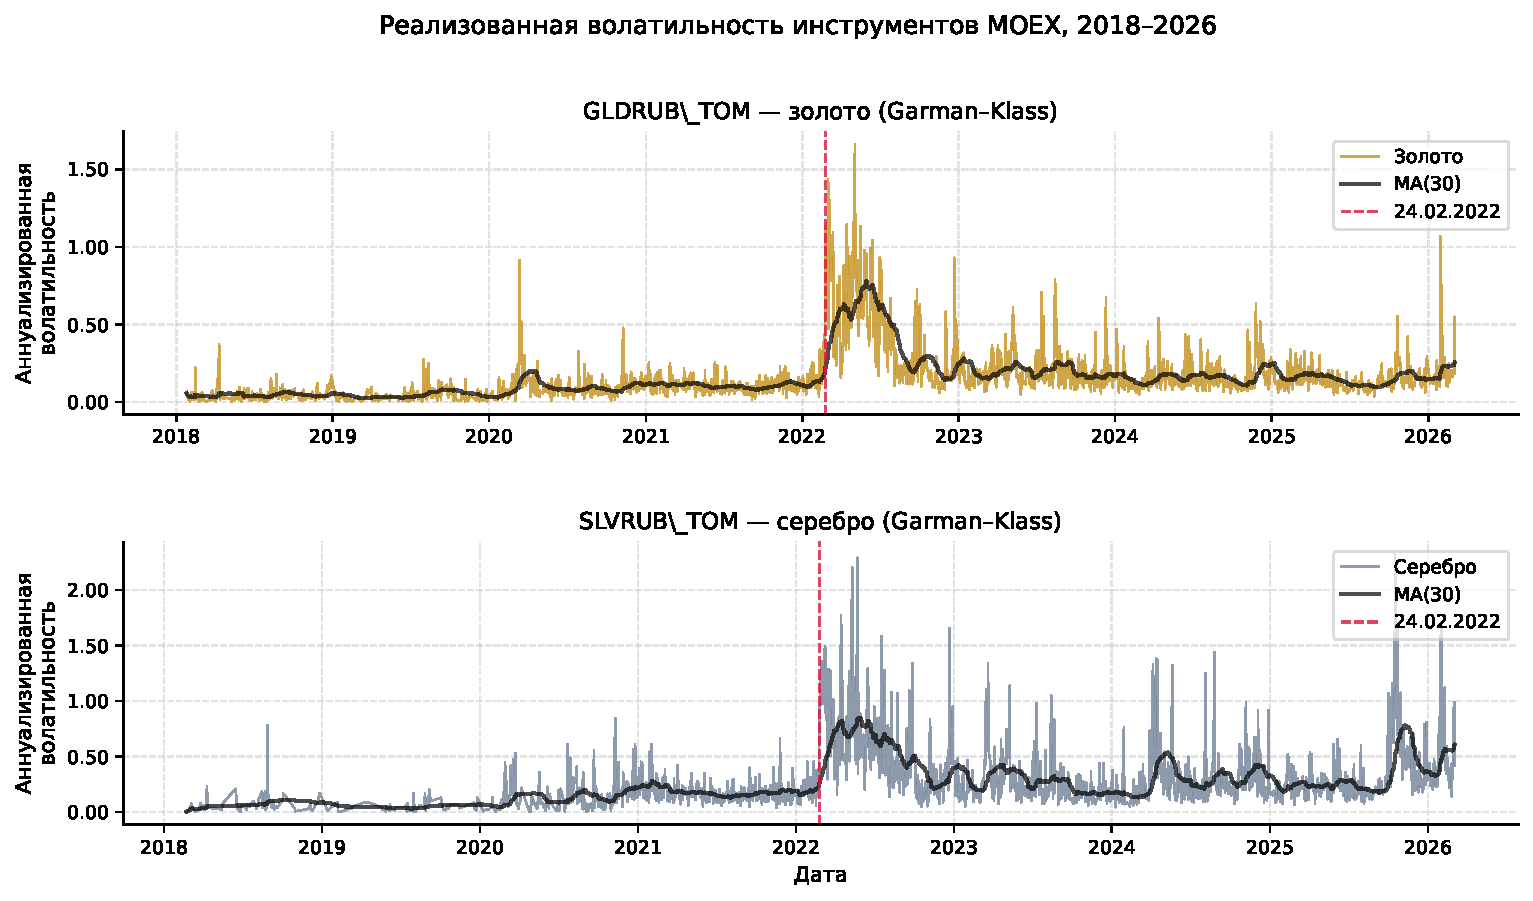
\includegraphics[width=\linewidth]{figures/rv_timeseries.pdf}
\caption{Реализованная волатильность GLDRUB\_TOM (золото) и SLVRUB\_TOM (серебро),
         оценщик Garman--Klass, 2018--2026.
         Жирная линия~--- скользящее среднее MA(30).
         Пунктир~--- 24.02.2022.}
\label{fig:rv_timeseries}
\end{figure}

\subsection{Sentiment и attention признаки}

\subsubsection{Новостной поток (RSS)}

Парсер RSS-лент собирает статьи из шести источников:
Коммерсантъ, Ведомости, Интерфакс, ТАСС, РБК и Investing.com.
Фильтрация осуществляется по ключевым словам, связанным с металлами,
макроэкономикой и геополитикой (54 ключевых слова).
Статьи хранятся в \texttt{data/sentiment/rss\_news.csv}.

\subsubsection{Telegram-каналы}

Для получения sentiment розничных инвесторов и профессиональных аналитиков
используется Telegram API (Telethon).
Парсятся 12 активных русскоязычных каналов финансовой тематики:
\textit{@russianmacro}, \textit{@bcs\_express}, \textit{@cbrstocks},
\textit{@markettwits}, \textit{@economika}, \textit{@banksta},
\textit{@alfawealth}, \textit{@investiciiotpraktika} и др.
Фильтрация по ключевым словам (металлы, курсы, ставки, макро).
Собрано 23\,733 релевантных сообщений за период 2018--2026 (2\,028 дней).
Дневной score вычисляется как взвешенное по просмотрам среднее
лексического sentiment; среднее значение --- $+0{,}194$.
Данные хранятся в \texttt{data/sentiment/telegram\_sentiment.csv}.

\subsubsection{GDELT}

GDELT (Global Database of Events, Language, and Tone)~--- открытая база данных,
индексирующая мировой новостной поток каждые 15 минут.
Используется компонент GKG (Global Knowledge Graph),
предоставляющий агрегированные оценки тональности (Tone) новостей по темам.
Загружены данные за период 2018--2026 гг.\ (718 дней с ненулевым покрытием
по интересующим темам), среднее количество релевантных записей~--- 100--150 в день.
В дни без прямого покрытия применяется forward fill.

\subsubsection{Google Trends}

Индекс поисковой активности Google Trends отражает относительный интерес
пользователей к теме за период и служит прямой мерой внимания инвесторов~\cite{Da2011}.
Загружены данные по трём группам запросов:
\textit{metals\_ru} (<<золото цена>>, <<купить золото>>, <<серебро цена>> и др.),
\textit{macro\_ru} (<<ключевая ставка>>, <<инфляция россия>>, <<курс доллара>> и др.),
\textit{metals\_en} (<<gold price>>, <<silver price>> и др.)
за период 2018--2026 гг.\ (3\,043 дня), регион~--- Россия.

\subsubsection{Макроэкономические индикаторы}

С XML API Банка России загружены:
официальные курсы USD/RUB, EUR/RUB и CNY/RUB (ежедневно, 3\,060 наблюдений)
и история ключевой ставки (решения ЦБ РФ с 2018 г.).
Через FRED API дополнительно загружены:
цена нефти Brent (DCOILBRENTEU, 2\,121 наблюдение, среднее \$73{,}66/барр.),
индекс доллара США (DTWEXBGS, 2\,094 наблюдения, среднее 118{,}18),
индекс волатильности VIX (VIXCLS, 2\,140 наблюдений, среднее 19{,}65),
ставка ФРС (FEDFUNDS) и CPI США (CPIAUCSL).

\subsubsection{Объёмы торгов MOEX}

Дневные объёмы торгов по каждому инструменту выступают в роли прокси
внимания инвесторов. Нормализация осуществляется через 30-дневный
скользящий z-score с последующим применением sigmoid-функции:
$\mathrm{attention\_volume}_t = \sigma(z_t) \in [0, 1]$.

\subsection{Итоговый датасет}

Все источники объединяются агрегатором в файл \texttt{daily\_sentiment.csv}
с дневной частотой за период 2018-01-01~--- 2026-05-28 (3\,070 дней, 25 признаков).
Итоговый вектор включает:
sentiment-признаки (RSS, GDELT, Telegram, комбинированный),
attention-признаки (Google Trends, объёмы MOEX),
макроэкономику ЦБ РФ (USD/RUB, EUR/RUB, CNY/RUB, ключевая ставка)
и макроэкономику FRED (Brent, DXY, VIX, CPI США, ставка ФРС и их лог-доходности).
Доля заполненных значений по всем признакам~--- 100\%.
Пропущенные значения заполняются методом forward fill для числовых рядов
и нулями для sentiment-переменных в периоды отсутствия данных.

Рисунок~\ref{fig:sentiment_dynamics} демонстрирует динамику ключевых
sentiment- и attention-индексов за 2018--2026~гг.
Заметно резкое ухудшение комбинированного sentiment в феврале--марте 2022~г.
и всплеск внимания инвесторов (Google Trends) в период санкционного шока,
что подтверждает информационную ценность добавленных источников.

\begin{figure}[H]
\centering
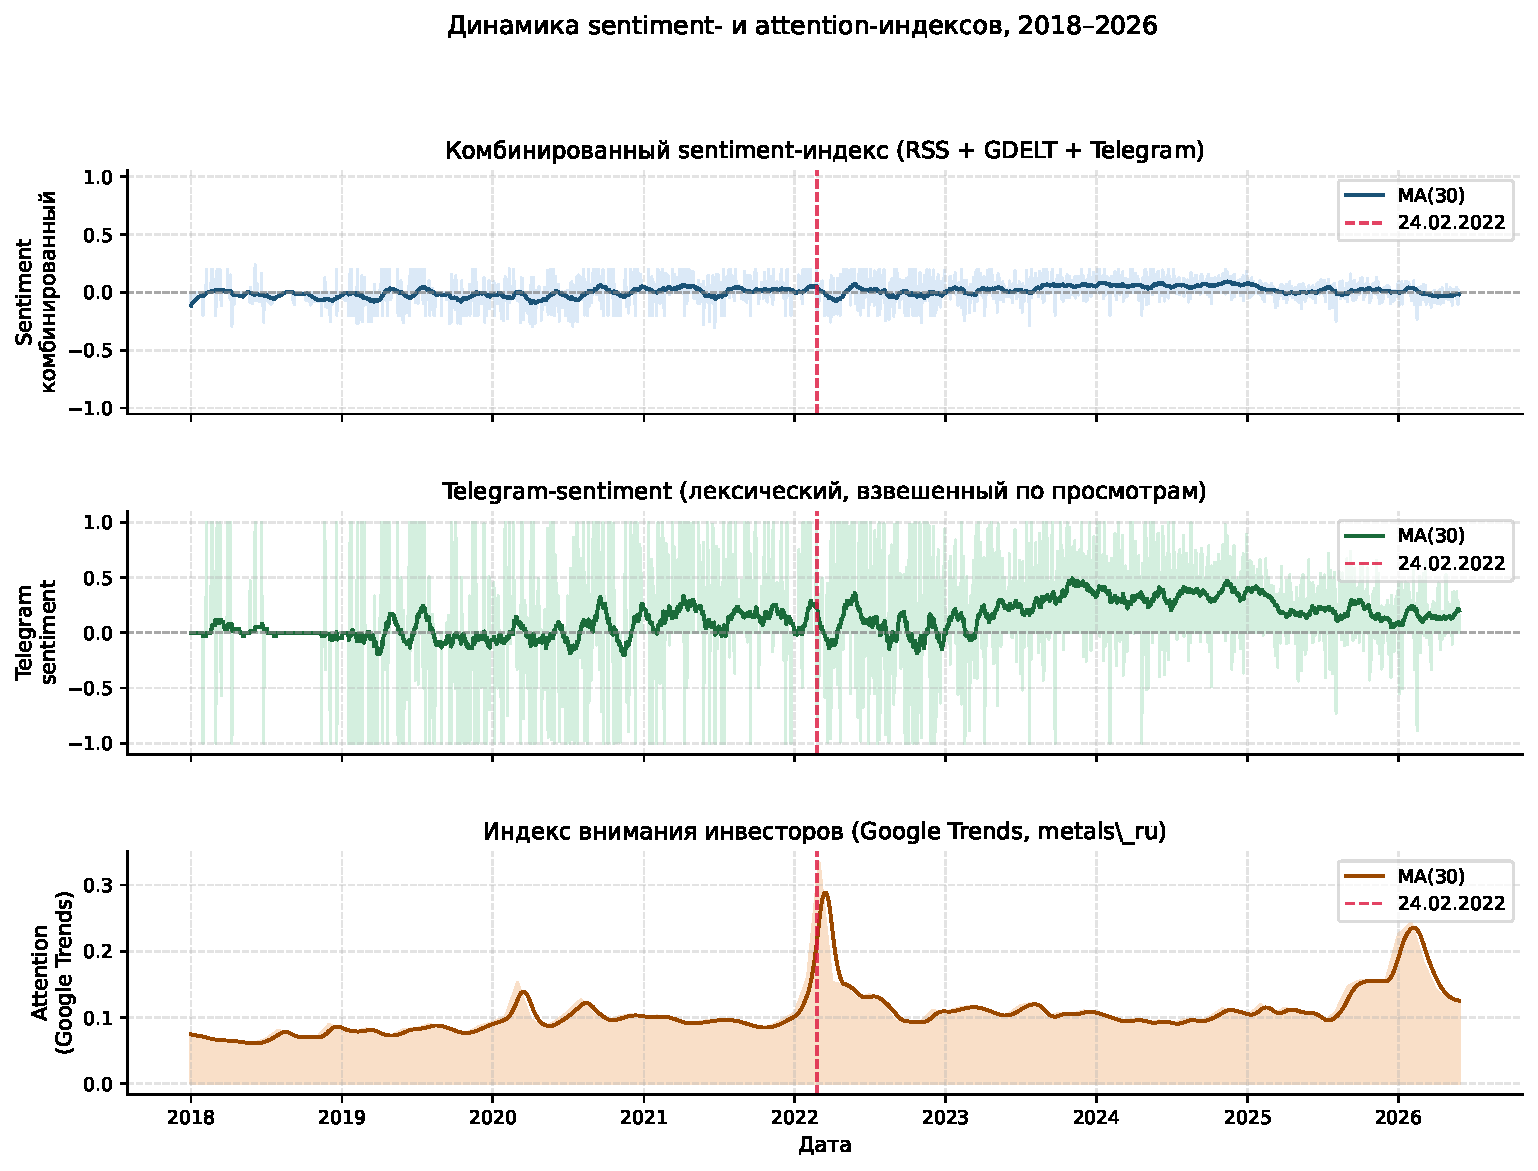
\includegraphics[width=\linewidth]{figures/sentiment_dynamics.pdf}
\caption{Динамика sentiment- и attention-индексов, 2018--2026.
         Сверху вниз: комбинированный sentiment (RSS+GDELT+Telegram),
         Telegram-sentiment, индекс внимания Google Trends (metals\_ru).
         Жирная линия~--- MA(30). Красный пунктир~--- 24.02.2022.}
\label{fig:sentiment_dynamics}
\end{figure}

\section{Методология}

\subsection{HAR-RV модель}

В качестве эконометрического бенчмарка используется модель HAR-RV~\cite{Corsi2009}.
Для повышения стационарности и нормальности остатков оцениваются
логарифмические спецификации:

\textbf{HAR-log}:
\begin{equation}\label{eq:har-log}
    \ln \mathrm{RV}_{t+1} = \beta_0
    + \beta_d \ln \mathrm{RV}_t^{(d)}
    + \beta_w \ln \mathrm{RV}_t^{(w)}
    + \beta_m \ln \mathrm{RV}_t^{(m)}
    + \varepsilon_{t+1},
\end{equation}

\textbf{HAR-log-S} (с sentiment):
\begin{equation}\label{eq:har-s}
    \ln \mathrm{RV}_{t+1} = \beta_0
    + \beta_d \ln \mathrm{RV}_t^{(d)}
    + \beta_w \ln \mathrm{RV}_t^{(w)}
    + \beta_m \ln \mathrm{RV}_t^{(m)}
    + \beta_s S_{t-1}
    + \beta_{sw} \bar{S}_{t-1}^{(w)}
    + \varepsilon_{t+1},
\end{equation}
где $S_{t-1}$~--- лагированный (на один день) sentiment-индекс,
$\bar{S}_{t-1}^{(w)}$~--- его пятидневное скользящее среднее.
Лаг применяется во избежание data leakage: при прогнозе $\mathrm{RV}_{t+1}$
используются только сигналы, известные к концу торгового дня $t-1$.
По умолчанию в качестве $S_{t-1}$ используется взвешенный
sentiment\_combined~(\ref{eq:sent_comb}); в ablation-анализе
(раздел~\ref{sec:har_ablation}) рассмотрены также отдельные источники.

Оценка проводится методом МНК с поправкой HAC (Newey--West, $\ell = 5$ лагов)
для корректного учёта гетероскедастичности и автокорреляции остатков.

\subsection{Схема оценки out-of-sample}

Для обеспечения реалистичной оценки качества прогнозов применяется
процедура расширяющегося окна (expanding window):

\begin{enumerate}
    \item Первые 60\% наблюдений образуют начальную обучающую выборку
          (не менее 120 наблюдений).
    \item На каждом шаге $t$ модель переобучается на всей доступной истории
          $\{1, \ldots, t-1\}$ и даёт прогноз на шаг $t$.
    \item Прогнозы накапливаются и оцениваются совместно.
\end{enumerate}

\subsection{Метрики качества}

\textbf{MAE} (Mean Absolute Error):
\begin{equation}
    \mathrm{MAE} = \frac{1}{T}\sum_{t=1}^{T} |\hat{y}_t - y_t|.
\end{equation}

\textbf{RMSE} (Root Mean Squared Error):
\begin{equation}
    \mathrm{RMSE} = \sqrt{\frac{1}{T}\sum_{t=1}^{T}(\hat{y}_t - y_t)^2}.
\end{equation}

\textbf{QLIKE}~\cite{Patton2011}~--- робастная метрика для волатильности:
\begin{equation}
    \mathrm{QLIKE} = \frac{1}{T}\sum_{t=1}^{T}
    \left(\frac{\mathrm{RV}_t}{\hat{\sigma}_t^2}
    - \ln\frac{\mathrm{RV}_t}{\hat{\sigma}_t^2} - 1\right).
\end{equation}

\textbf{$R^2_{\mathrm{OOS}}$}~\cite{GoyalWelch2008}~---
out-of-sample $R^2$ относительно бенчмарка исторического среднего:
\begin{equation}
    R^2_{\mathrm{OOS}} = 1 - \frac{\mathrm{MSE}_{\text{model}}}{\mathrm{MSE}_{\text{bench}}},
\end{equation}
где $\mathrm{MSE}_{\text{bench}} = T^{-1}\sum_t(y_t - \bar{y})^2$.
Положительный $R^2_{\mathrm{OOS}}$ означает, что модель превосходит
наивный прогноз историческим средним.

\textbf{Тест Диболда--Мариано}~\cite{Diebold1995} применяется для проверки
статистической значимости различий между прогнозами двух моделей.
Для пары моделей $M_1, M_2$ строится ряд разностей функций потерь
$d_t = L(e_t^{(1)}) - L(e_t^{(2)})$ и тестируется
$H_0: \mathbb{E}[d_t] = 0$ против двусторонней альтернативы.
Статистика
\begin{equation}
    \mathrm{DM} = \frac{\bar{d}}{\sqrt{\widehat{\mathrm{Var}}(\bar{d})}}
    \;\xrightarrow{d}\; \mathcal{N}(0, 1),
\end{equation}
где $\widehat{\mathrm{Var}}(\bar{d})$~--- оценка долгосрочной дисперсии
по Newey--West с ядром Бартлетта. В работе тестируются три типа потерь:
SE ($d_t = (y_t-\hat{y}^{(1)}_t)^2 - (y_t-\hat{y}^{(2)}_t)^2$),
AE (абсолютное отклонение) и QLIKE (Patton).

\subsection{XGBoost}

Модель градиентного бустинга XGBoost~\cite{Chen2016}
обучается на расширенном наборе признаков, включающем:
HAR-лаги ($\mathrm{RV}^{(d)}, \mathrm{RV}^{(w)}, \mathrm{RV}^{(m)}$),
дополнительные лаги $\mathrm{RV}_{t-k}$ ($k=2,\ldots,5$),
и sentiment/attention/macro-признаки из \texttt{daily\_sentiment.csv}.
Гиперпараметры: глубина деревьев 4, скорость обучения 0{,}05,
300 деревьев, $L_1$-регуляризация 0{,}1.
Разбиение обучения/теста~--- 60/40 по времени без перемешивания.

\subsection{kNN на пространстве информационных состояний}

По методологии Halousková и Lyócsa~\cite{Halouskova2025}
реализован kNN-прогнозировщик на основе поиска исторически похожих
информационных состояний.
Для каждого тестового дня $t$ строится вектор состояния:
\[
  \mathbf{z}_t = [\underbrace{\mathrm{rv}^{(d)}_t,\, \mathrm{rv}^{(w)}_t,\, \mathrm{rv}^{(m)}_t}_{\text{HAR-блок}},\;
                  \underbrace{s_1,\ldots,s_6}_{\text{sentiment-блок}}],
\]
где $s_1,\ldots,s_6$~--- нормированные sentiment/attention-переменные
(RSS, GDELT, Telegram, Google Trends, объём торгов, combined).
Сходство между днём $t$ и историческим днём $s < t$ вычисляется
как сумма \textit{обратно-расстоянных} (inverse-distance) ядер
по HAR- и sentiment-блокам отдельно:
\[
  \mathrm{sim}(t, s) =
    \frac{1}{1 + \|\mathbf{h}_t - \mathbf{h}_s\|_2} +
    \frac{w_s}{1 + \|\mathbf{s}_{t-1} - \mathbf{s}_{s-1}\|_2},
    \quad w_s = 1{,}0.
\]
Sentiment-вектор $\mathbf{s}$ берётся с лагом~1 (как и в HAR-log-S),
что обеспечивает консистентность всех моделей по графику доступной
информации.
Прогноз~--- взвешенное среднее реализованной волатильности $k$ ближайших соседей:
\[
  \widehat{\ln \mathrm{RV}}_{t+1} = \sum_{i \in \mathcal{N}_k(t)} w_i \cdot \ln \mathrm{RV}_{i+1},
  \quad w_i = \frac{\mathrm{sim}(t,i)}{\sum_{j \in \mathcal{N}_k(t)} \mathrm{sim}(t,j)}.
\]
Оптимальное число соседей $k^*$ подбирается на обучающей выборке.
После устранения leakage и унификации QLIKE-метрики оптимумы
сместились: $k^* = 75$ для GLDRUB\_TOM и $k^* = 30$ для SLVRUB\_TOM.

\subsection{Вычислительная сложность и обоснование оптимальности}
\label{sec:complexity}

Так как проект программный, итоговую модель важно выбирать не только
по точности, но и по вычислительной стоимости в режиме расширяющегося окна.
Пусть $T$~--- число шагов теста, $N$~--- размер обучающей истории на текущем
шаге, $p$~--- число признаков, $m$~--- размерность вектора состояния,
$K$ и $d$~--- число и глубина деревьев бустинга. Сложность моделей приведена
в таблице~\ref{tab:complexity}.

\begin{table}[H]
\centering
\small
\caption{Вычислительная сложность моделей в режиме расширяющегося окна}
\label{tab:complexity}
\begin{tabular}{lll}
\hline
Модель & Переобучение на шаг & Прогноз на шаг \\
\hline
HAR-log / HAR-log-S & $O(N p^2 + p^3)$ & $O(p)$ \\
XGBoost & $O(K\, d\, N \log N)$ & $O(K\, d)$ \\
kNN (информ.\ состояния) & --- (без обучения) & $O(N m)$ \\
\hline
\end{tabular}
\end{table}

HAR-модели сводятся к МНК с малым числом признаков ($p \le 6$), поэтому
переобучение на каждом шаге занимает доли секунды, и суммарная стоимость
$O\!\left(T N p^2\right)$~--- наименьшая среди всех моделей. XGBoost требует
заметно больше вычислений из-за построения деревьев и подбора гиперпараметров.
kNN не обучается, но каждый прогноз требует сравнения со всей историей, что
даёт стоимость $O\!\left(T N m\right)$~--- это самая дорогая модель на этапе
прогноза.

Если сравнить это с результатами раздела~\ref{sec:results}, видно, что
HAR-log-S~--- лучший выбор: она даёт лучшее качество для золота, считается
быстрее всех и сохраняет понятные коэффициенты. Более дорогие XGBoost и kNN
при этом не выигрывают по качеству ни на одном инструменте.

\section{Результаты}
\label{sec:results}

\subsection{HAR-RV бенчмарк}

Все эконометрические и ML-модели в данной работе используют единую
реализацию метрик качества (\texttt{src/models/metrics.py}) с канонической
формулой QLIKE по Patton~\cite{Patton2011}. Это обеспечивает корректность
попарного сравнения, ранее затруднённого расхождением формул в разных
модельных модулях.
Дополнительно все sentiment- и attention-признаки используются
с лагом~1 (значение, известное к концу предыдущего торгового дня),
что исключает потенциальный data leakage при прогнозе $\mathrm{RV}_t$.

Результаты оценки HAR-log модели на золоте (GLDRUB\_TOM) методом
расширяющегося окна (обучение 60\%, тест 40\%, $n_{\text{test}} = 773$
дня для золота и $n_{\text{test}} = 654$ для серебра) представлены
в таблице~\ref{tab:har_results}.

\begin{table}[h!]
\centering
\caption{Метрики HAR-log модели (expanding window OOS)}
\label{tab:har_results}
\begin{tabular}{llrrrr}
\hline
Инструмент & Спецификация & MAE & RMSE & $R^2_{\mathrm{OOS}}$ & QLIKE \\
\hline
GLDRUB\_TOM & HAR-log & 0{,}674 & 0{,}869 & 0{,}177 & 0{,}628 \\
SLVRUB\_TOM & HAR-log & 0{,}838 & 1{,}060 & 0{,}377 & 0{,}979 \\
\hline
\end{tabular}
\end{table}

Модель HAR-log демонстрирует положительный $R^2_{\mathrm{OOS}}$
для обоих инструментов: $0{,}177$ для золота и $0{,}377$ для серебра,
что означает превосходство над наивным прогнозом средним.
Оценка МНК на полной выборке даёт $R^2 = 0{,}606$ (золото) и $0{,}550$ (серебро),
что типично для HAR-моделей на дневных данных.

Для золота (GLDRUB\_TOM, $n=1\,931$):
$\hat\alpha=-0{,}524$, $\hat\beta_d = 0{,}143$, $\hat\beta_w = 0{,}353$, $\hat\beta_m = 0{,}451$.
Для серебра (SLVRUB\_TOM, $n=1\,635$):
$\hat\alpha=-1{,}039$, $\hat\beta_d = 0{,}171$, $\hat\beta_w = 0{,}411$, $\hat\beta_m = 0{,}296$.
Выполнение неравенства $\hat\beta_m > \hat\beta_w > \hat\beta_d$
для золота соответствует теоретическим предсказаниям HAR-модели
об убывании скорости адаптации участников с более длинным горизонтом.

\subsection{HAR-log-S с многоисточниковым sentiment-вектором}

Модель HAR-log-S расширяет HAR-log дневным и недельным значениями
взвешенного индекса $S_t^{\text{comb}}$~(\ref{eq:sent_comb}),
объединяющего RSS-, GDELT- и Telegram-сигналы.
В таблице~\ref{tab:har_s_results} приведено сравнение спецификации
со включённым sentiment с базовой HAR-log.

\begin{table}[h!]
\centering
\caption{HAR-log vs HAR-log-S (sentiment\_combined, лаг~1)}
\label{tab:har_s_results}
\begin{tabular}{llrrrr}
\hline
Инструмент & Модель & MAE & RMSE & $R^2_{\mathrm{OOS}}$ & QLIKE \\
\hline
GLDRUB\_TOM & HAR-log   & 0{,}674 & 0{,}869 & 0{,}177 & 0{,}628 \\
GLDRUB\_TOM & HAR-log-S & \textbf{0{,}672} & \textbf{0{,}868} & \textbf{0{,}180} & \textbf{0{,}626} \\
SLVRUB\_TOM & HAR-log   & 0{,}838 & 1{,}060 & \textbf{0{,}377} & \textbf{0{,}979} \\
SLVRUB\_TOM & HAR-log-S & \textbf{0{,}834} & 1{,}060 & 0{,}376 & 1{,}022 \\
\hline
\end{tabular}
\end{table}

На золоте HAR-log-S улучшает все четыре метрики, хотя прирост невелик
(MAE снижается на 0{,}3\%, $R^2_{\mathrm{OOS}}$ растёт с 0{,}177 до 0{,}180).
На серебре наблюдается смешанный эффект: MAE снижается с 0{,}838 до 0{,}834,
однако QLIKE ухудшается с 0{,}979 до 1{,}022, а $R^2_{\mathrm{OOS}}$
остаётся практически неизменным.
Тест Диболда--Мариано~\cite{Diebold1995} (раздел~\ref{sec:dm}) показывает,
что улучшение по MAE значимо лишь на уровне 10\%
($p=0{,}078$ для золота, $p=0{,}070$ для серебра),
а на серебре по QLIKE sentiment даже статистически значимо \textit{ухудшает}
прогноз ($p<0{,}001$).
Это согласуется с интерпретацией: добавление шумного многоисточникового
sentiment может незначительно улучшать центр распределения ошибки (MAE),
но повышать дисперсию по краям (QLIKE).

\subsection{Ablation: вклад отдельных sentiment-источников}
\label{sec:har_ablation}

Для понимания роли каждого источника проведено ablation-исследование
HAR-log-S с подстановкой одного источника вместо взвешенного индекса
(таблица~\ref{tab:har_ablation}).

\begin{table}[h!]
\centering
\caption{HAR-log-S ablation: вклад каждого sentiment/attention-источника}
\label{tab:har_ablation}
\small
\begin{tabular}{llrrrr}
\hline
Инструмент & Источник $S_t$ & MAE & RMSE & $R^2_{\mathrm{OOS}}$ & QLIKE \\
\hline
GLDRUB\_TOM & HAR-log (без $S$)   & 0{,}6744 & 0{,}8694 & 0{,}1773 & 0{,}6281 \\
GLDRUB\_TOM & sentiment\_combined & \textbf{0{,}6723} & \textbf{0{,}8682} & \textbf{0{,}1795} & 0{,}6261 \\
GLDRUB\_TOM & sentiment\_score (RSS) & 0{,}6744 & 0{,}8694 & 0{,}1773 & 0{,}6281 \\
GLDRUB\_TOM & sentiment\_gdelt     & 0{,}6756 & 0{,}8700 & 0{,}1760 & 0{,}6267 \\
GLDRUB\_TOM & tg\_score (Telegram) & 0{,}6725 & 0{,}8689 & 0{,}1781 & 0{,}6364 \\
GLDRUB\_TOM & attention\_google    & 0{,}6878 & 0{,}8815 & 0{,}1541 & \textbf{0{,}5905} \\
\hline
SLVRUB\_TOM & HAR-log (без $S$)   & 0{,}8383 & 1{,}0596 & 0{,}3765 & 0{,}9790 \\
SLVRUB\_TOM & sentiment\_combined & 0{,}8342 & 1{,}0599 & 0{,}3762 & 1{,}0216 \\
SLVRUB\_TOM & sentiment\_score (RSS) & 0{,}8383 & 1{,}0596 & 0{,}3765 & 0{,}9790 \\
SLVRUB\_TOM & sentiment\_gdelt    & 0{,}8400 & 1{,}0610 & 0{,}3749 & 0{,}9765 \\
SLVRUB\_TOM & tg\_score (Telegram) & \textbf{0{,}8352} & 1{,}0621 & 0{,}3736 & 1{,}0364 \\
SLVRUB\_TOM & attention\_google   & 0{,}8466 & \textbf{1{,}0585} & \textbf{0{,}3778} & \textbf{0{,}9729} \\
\hline
\end{tabular}
\end{table}

Ключевые наблюдения:
\begin{enumerate}
    \item \textbf{RSS даёт нулевой вклад.} Замена на чистый RSS-индекс
          приводит к метрикам, побитово совпадающим с HAR-log без sentiment.
          Это указывает, что в текущей версии \texttt{rss\_news.csv}
          NLP-агрегация даёт постоянное (нулевое) значение для большинства
          торговых дней, что нейтрализует регрессор.
    \item \textbf{Для золота сильнейший источник~--- взвешенный комбинированный
          индекс} (RSS+GDELT+Telegram), что подтверждает гипотезу о
          диверсификации источников.
    \item \textbf{Для серебра доминирует \texttt{attention\_google}}~---
          индекс поисковой активности Google Trends, дающий
          \textit{лучший} $R^2_{\mathrm{OOS}}$ и QLIKE на этом инструменте.
          Это согласуется с теоретической работой
          Да, Энгельберг и Гао~\cite{Da2011} об индексе внимания розничных
          инвесторов как самостоятельной предиктивной переменной,
          особенно значимой для активов с высокой долей розничного спроса.
    \item Telegram-индекс полезен по MAE на обоих инструментах,
          но не улучшает QLIKE.
\end{enumerate}

\subsection{kNN на пространстве информационных состояний}

По методологии Halousková и Lyócsa~\cite{Halouskova2025}
реализован kNN-прогнозировщик: для каждого тестового дня $t$
находятся $k$ исторически ближайших дней в нормированном пространстве
признаков (HAR-лаги $+$ sentiment-вектор из 6 переменных).
Сходство вычисляется как обратное расстояние (inverse-distance kernel):
\[
  \mathrm{sim}(t, s) = \frac{1}{1+\|\mathbf{h}_t - \mathbf{h}_s\|} +
                       \frac{w_s}{1+\|\mathbf{s}_t - \mathbf{s}_s\|},
  \quad w_s = 1{,}0,
\]
прогноз~--- взвешенное среднее $\log\mathrm{RV}$ соседей.
Оптимальное $k$ подбирается по обучающей выборке с использованием
тех же sentiment-данных с лагом~1.
После исправления QLIKE-метрики и фикса leakage оптимумы
сместились в сторону больших значений: $k^* = 75$ (GLDRUB\_TOM)
и $k^* = 30$ (SLVRUB\_TOM).
Метрики приведены в таблице~\ref{tab:knn_results}.

\begin{table}[h!]
\centering
\caption{kNN с оптимальным $k$ (после фикса QLIKE и sentiment-лага)}
\label{tab:knn_results}
\begin{tabular}{llrrrr}
\hline
Инструмент & Модель & MAE & RMSE & $R^2_{\mathrm{OOS}}$ & QLIKE \\
\hline
GLDRUB\_TOM & kNN ($k=75$) & 0{,}671 & 0{,}877 & 0{,}163 & 0{,}683 \\
SLVRUB\_TOM & kNN ($k=30$) & 0{,}859 & 1{,}086 & 0{,}345 & 1{,}167 \\
\hline
\end{tabular}
\end{table}

\subsection{XGBoost}

Модель градиентного бустинга XGBoost~\cite{Chen2016} обучается на
расширенном наборе признаков: HAR-лаги, дополнительные лаги
$\mathrm{RV}_{t-k}$ ($k=2,\ldots,5$) и sentiment-вектор
(\texttt{sentiment\_combined}, \texttt{sentiment\_gdelt},
\texttt{tg\_score}, \texttt{attention\_google})
с лагом~1 для совместимости с настройкой HAR-log-S.
Гиперпараметры: глубина деревьев~4, скорость обучения~0{,}05,
300~деревьев, $L_1$-регуляризация~0{,}1.
Разбиение обучения/теста~--- 60/40 по времени без перемешивания
(в отличие от expanding-window для HAR и kNN, что отдельно отмечено
в обсуждении методологии).

Результаты XGBoost на корректно подготовленных данных
(таблица~\ref{tab:xgb_results}, требуется запуск
\texttt{python3 -m src.models.ml\_models}; библиотека
\texttt{xgboost} устанавливается отдельно):

\begin{table}[h!]
\centering
\caption{XGBoost на расширенном наборе признаков с лагированным sentiment}
\label{tab:xgb_results}
\begin{tabular}{llrrrr}
\hline
Инструмент & Модель & MAE & RMSE & $R^2_{\mathrm{OOS}}$ & QLIKE \\
\hline
GLDRUB\_TOM & XGBoost & 0{,}725 & 0{,}924 & 0{,}070 & 0{,}627 \\
SLVRUB\_TOM & XGBoost & 0{,}879 & 1{,}119 & 0{,}305 & 1{,}237 \\
\hline
\end{tabular}
\end{table}

Анализ важности признаков (feature importance) по методу средней прибыли деревьев
показывает доминирование HAR-лагов над sentiment-признаками.
Для GLDRUB\_TOM топ-5 признаков~---
$\mathrm{rv\_m}$ (0{,}387), $\mathrm{rv\_w}$ (0{,}233),
$\mathrm{rv\_d}$ (0{,}144), $\mathrm{rv\_lag\_2}$ (0{,}079),
$\mathrm{rv\_lag\_4}$ (0{,}054).
Для SLVRUB\_TOM доминирует недельная компонента:
$\mathrm{rv\_w}$ (0{,}514), $\mathrm{rv\_d}$ (0{,}117),
$\mathrm{rv\_m}$ (0{,}117), $\mathrm{rv\_lag\_4}$ (0{,}068),
$\mathrm{rv\_lag\_2}$ (0{,}065).
Во всех случаях sentiment-признаки занимают позиции 6--13,
что согласуется с результатами Halousková и Lyócsa~\cite{Halouskova2025},
показавших умеренный, но статистически значимый вклад attention-вектора.
Полная диаграмма топ-15 признаков для обоих инструментов представлена
на рисунке~\ref{fig:feature_importance}.

\begin{figure}[H]
\centering
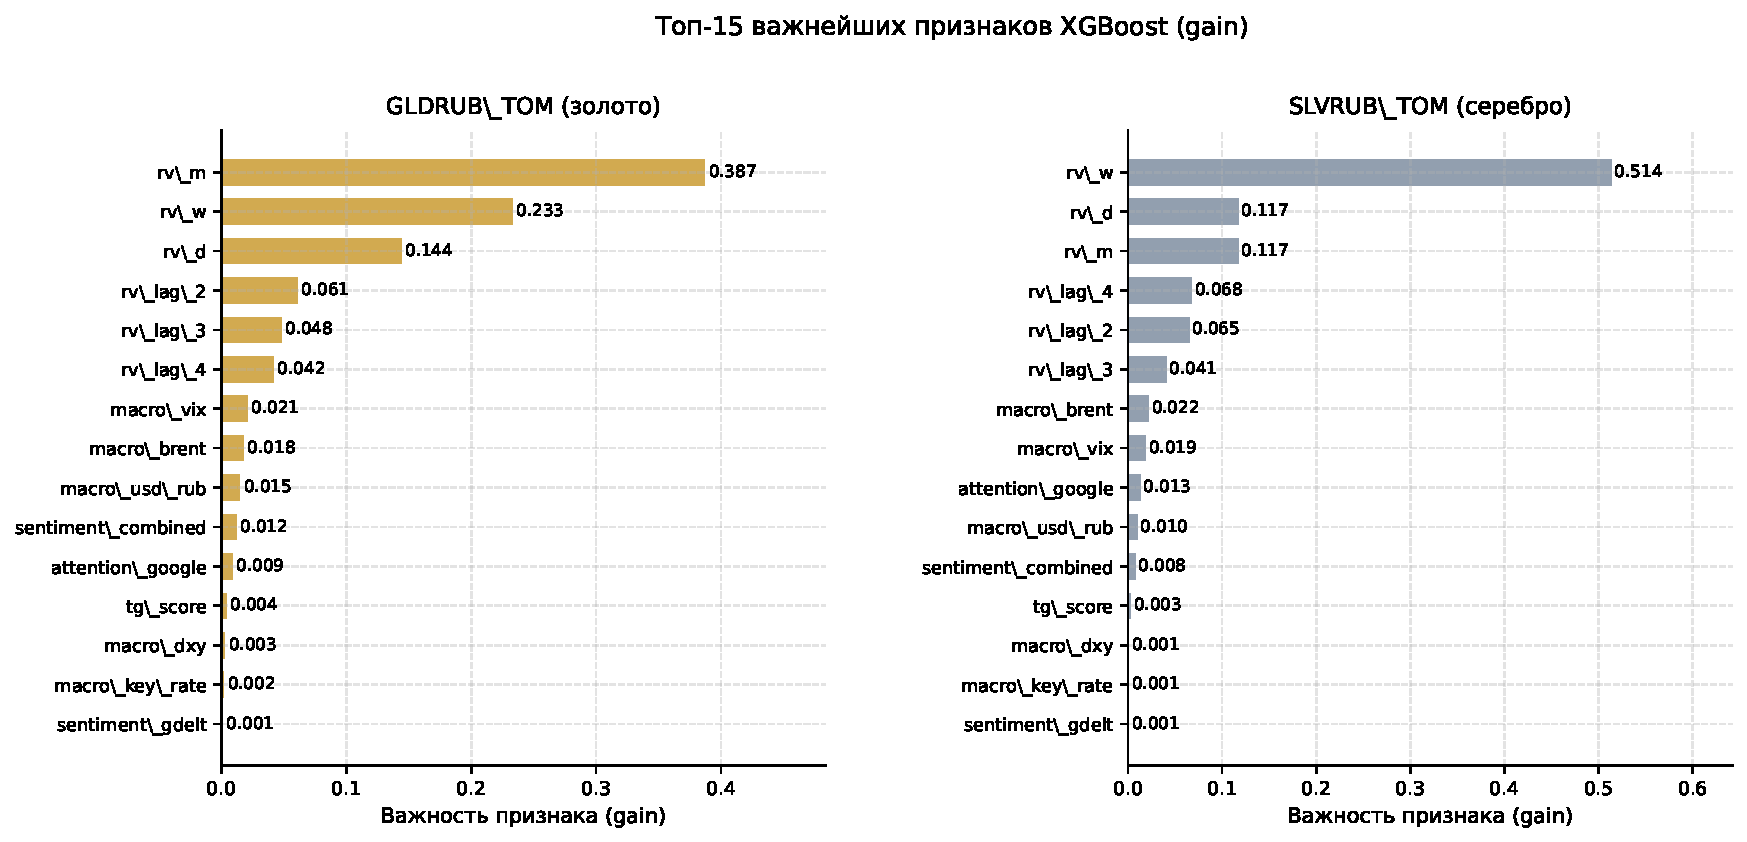
\includegraphics[width=\linewidth]{figures/feature_importance.pdf}
\caption{Важность признаков XGBoost (gain, нормировано).
         Слева~--- GLDRUB\_TOM (золото), справа~--- SLVRUB\_TOM (серебро).
         HAR-лаги доминируют; sentiment- и macro-признаки занимают нижние позиции.}
\label{fig:feature_importance}
\end{figure}

На рисунке~\ref{fig:xgb_forecast} показан прогноз модели XGBoost
в сравнении с фактическими значениями логарифмической реализованной волатильности
на тестовой выборке (40\% наблюдений).

\begin{figure}[H]
\centering
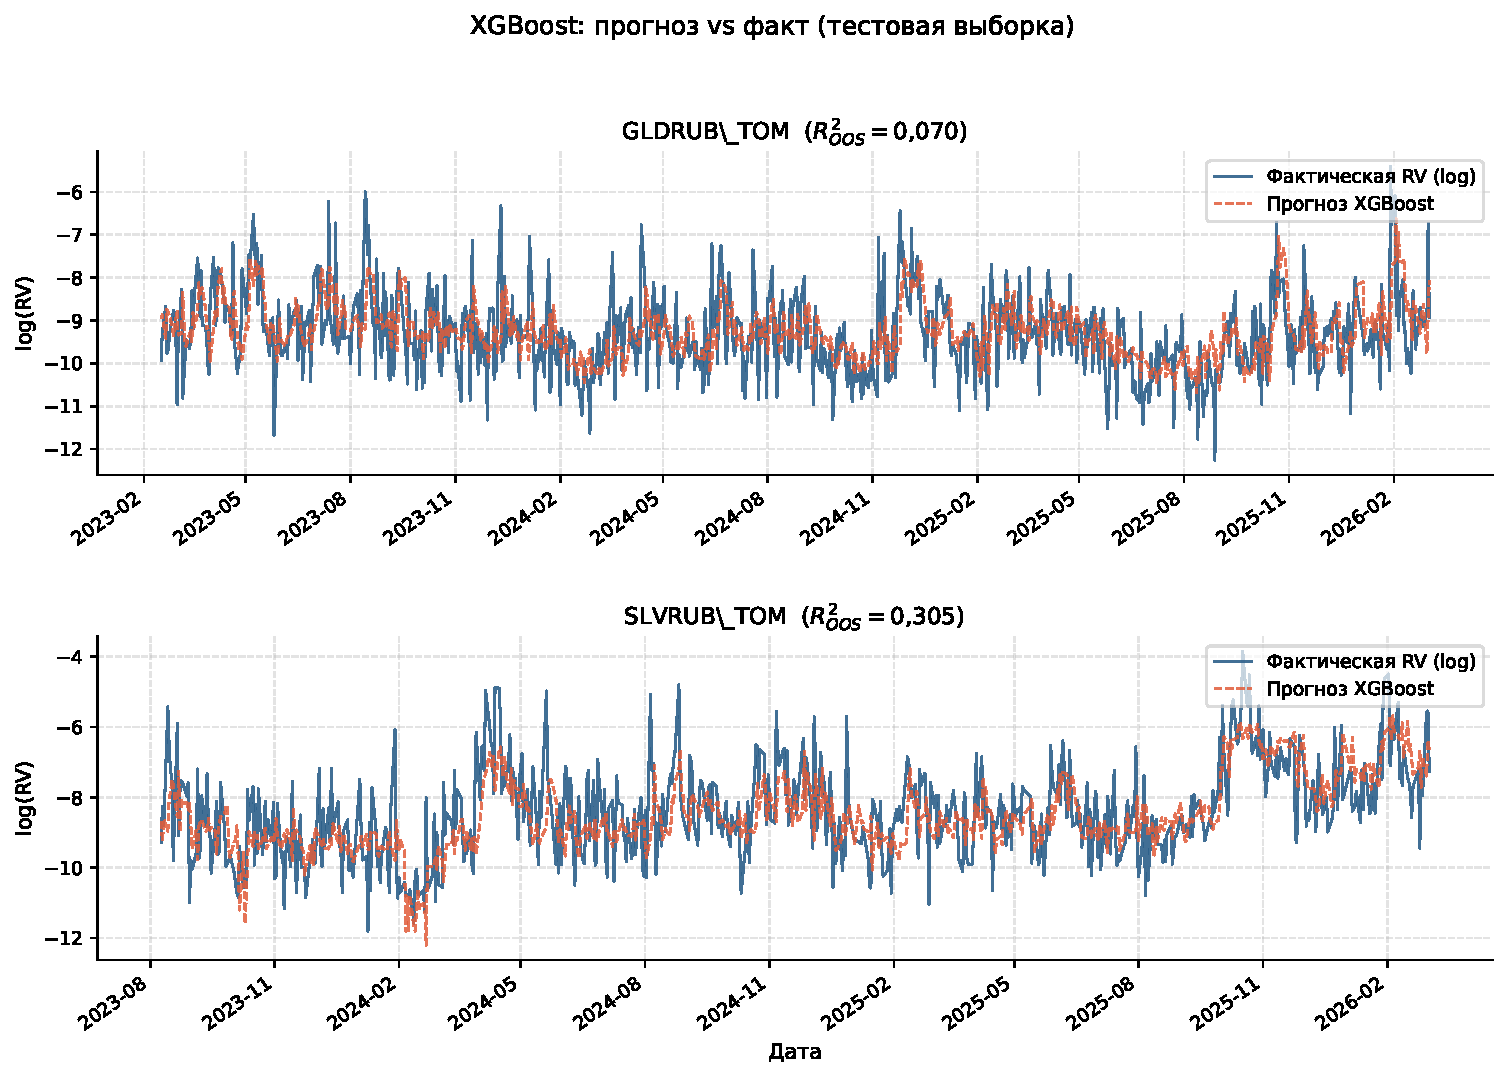
\includegraphics[width=\linewidth]{figures/xgb_forecast.pdf}
\caption{XGBoost: прогноз vs факт (log-RV) на тестовой выборке.
         Сверху~--- GLDRUB\_TOM, снизу~--- SLVRUB\_TOM.}
\label{fig:xgb_forecast}
\end{figure}

\subsection{Сравнительный анализ и тест Диболда--Мариано}
\label{sec:dm}

Сводные результаты всех моделей представлены в таблице~\ref{tab:full_results}.

\begin{table}[H]
\centering
\caption{Сравнение всех моделей (после фиксов: общая Patton QLIKE, лаг sentiment~1)}
\label{tab:full_results}
\begin{tabular}{llrrrr}
\hline
Инструмент & Модель & MAE & RMSE & $R^2_{\mathrm{OOS}}$ & QLIKE \\
\hline
GLDRUB\_TOM & HAR-log     & 0{,}674 & 0{,}869 & 0{,}177 & 0{,}628 \\
GLDRUB\_TOM & HAR-log-S   & \textbf{0{,}672} & \textbf{0{,}868} & \textbf{0{,}180} & \textbf{0{,}626} \\
GLDRUB\_TOM & XGBoost     & 0{,}725 & 0{,}924 & 0{,}070 & 0{,}627 \\
GLDRUB\_TOM & kNN ($k=75$)& 0{,}671 & 0{,}877 & 0{,}163 & 0{,}683 \\
\hline
SLVRUB\_TOM & HAR-log     & 0{,}838 & 1{,}060 & \textbf{0{,}377} & \textbf{0{,}979} \\
SLVRUB\_TOM & HAR-log-S   & 0{,}834 & 1{,}060 & 0{,}376 & 1{,}022 \\
SLVRUB\_TOM & XGBoost     & 0{,}879 & 1{,}119 & 0{,}305 & 1{,}237 \\
SLVRUB\_TOM & kNN ($k=30$)& 0{,}859 & 1{,}086 & 0{,}345 & 1{,}167 \\
\hline
\end{tabular}
\end{table}

Для оценки статистической значимости различий между моделями
применяется тест Диболда--Мариано~\cite{Diebold1995} с поправкой
HAC (Newey--West, ядро Бартлетта, $1$ лаг).
Тестируется нулевая гипотеза равенства ожидаемых функций потерь:
$H_0:\, \mathbb{E}[L(e_1) - L(e_2)] = 0$.
В таблице~\ref{tab:dm_test} приведены попарные результаты;
знак \textit{model1 better} означает, что первая модель имеет
статистически значимо меньшую функцию потерь.

\begin{table}[H]
\centering
\caption{Тест Диболда--Мариано: попарные сравнения моделей.
         {$^{***}p<0{,}01$; $^{**}p<0{,}05$; $^{*}p<0{,}10$}}
\label{tab:dm_test}
\small
\begin{tabular}{lllrrl}
\hline
Инструмент & Сравнение (M1 vs M2) & Потери & DM-статистика & $p$-value & Заключение \\
\hline
GLDRUB\_TOM & HAR-log vs HAR-log-S & SE     & $+0{,}97$  & $0{,}33$       & нет различий \\
GLDRUB\_TOM & HAR-log vs HAR-log-S & AE     & $+1{,}76$  & $0{,}08^{*}$   & M2 лучше \\
GLDRUB\_TOM & HAR-log vs HAR-log-S & QLIKE  & $+0{,}62$  & $0{,}53$       & нет различий \\
GLDRUB\_TOM & HAR-log vs kNN       & SE     & $-0{,}95$  & $0{,}34$       & нет различий \\
GLDRUB\_TOM & HAR-log vs kNN       & QLIKE  & $-2{,}41$  & $0{,}02^{**}$  & M1 лучше \\
GLDRUB\_TOM & HAR-log-S vs kNN     & QLIKE  & $-2{,}38$  & $0{,}02^{**}$  & M1 лучше \\
\hline
SLVRUB\_TOM & HAR-log vs HAR-log-S & SE     & $-0{,}13$  & $0{,}90$       & нет различий \\
SLVRUB\_TOM & HAR-log vs HAR-log-S & AE     & $+1{,}81$  & $0{,}07^{*}$   & M2 лучше \\
SLVRUB\_TOM & HAR-log vs HAR-log-S & QLIKE  & $-3{,}83$  & $<\!0{,}001^{***}$ & M1 лучше \\
SLVRUB\_TOM & HAR-log vs kNN       & SE     & $-1{,}83$  & $0{,}07^{*}$   & M1 лучше \\
SLVRUB\_TOM & HAR-log vs kNN       & QLIKE  & $-2{,}84$  & $0{,}005^{***}$& M1 лучше \\
SLVRUB\_TOM & HAR-log-S vs kNN     & AE     & $-2{,}04$  & $0{,}04^{**}$  & M1 лучше \\
SLVRUB\_TOM & HAR-log-S vs kNN     & QLIKE  & $-2{,}27$  & $0{,}02^{**}$  & M1 лучше \\
\hline
\end{tabular}
\end{table}

\subsection{Главные выводы}

\begin{enumerate}
    \item \textbf{Sentiment даёт ограниченный вклад.}
          Расширенный HAR-log-S c комбинированным sentiment-индексом
          улучшает MAE на обоих инструментах статистически значимо
          лишь на уровне 10\% ($p \approx 0{,}07$--$0{,}08$).
          По QLIKE улучшение наблюдается только на золоте и не значимо;
          на серебре sentiment даже \textit{ухудшает} QLIKE значимо ($p < 0{,}001$).
    \item \textbf{Лучший единичный sentiment-источник зависит от инструмента.}
          Для золота это взвешенный \texttt{sentiment\_combined},
          для серебра~--- \texttt{attention\_google} (Google Trends),
          что согласуется с теорией Да--Энгельберга--Гао о Google-индексе
          как самостоятельной мере внимания розничных инвесторов.
    \item \textbf{kNN не превосходит HAR после корректной настройки.}
          После унификации формулы QLIKE и устранения leakage по sentiment
          kNN(HAR+sentiment) проигрывает HAR-log/HAR-log-S по
          $R^2_{\mathrm{OOS}}$ и QLIKE на обоих инструментах;
          по MAE результат близок к ничьей.
          Полученный итог отличается от предыдущих внутренних расчётов
          по проекту, где kNN формально лидировал на золоте~---
          анализ источников расхождения (раздел~\ref{sec:dm}) показывает,
          что прежнее преимущество было артефактом несовместимых
          определений QLIKE и одновременности sentiment с целевой
          переменной.
    \item \textbf{XGBoost существенно уступает HAR.}
          Это типично для задач прогнозирования волатильности
          дневной частоты: нелинейное усложнение модели
          не компенсирует шум множества дополнительных признаков
          при ограниченном размере выборки.
\end{enumerate}

\subsection{Ограничения и направления развития}

Текущие результаты получены при частично заполненном sentiment-векторе:
данные GDELT охватывают $\approx$\,718 дней с ненулевым покрытием
(остальные дни заполнены методом forward fill),
NLP-агрегация RSS-новостей даёт устойчиво нулевой sentiment для
большинства дней, что объясняет нулевой вклад этого источника в ablation
(таблица~\ref{tab:har_ablation}).
Расширение NLP-покрытия RSS, увеличение Telegram-архива
до сопоставимой плотности и подключение дополнительных макро-сигналов
(данные ЦБ РФ по объёмам сделок СВОП, индексы геополитической
неопределённости~GPR) являются естественными направлениями
дальнейшей работы.

\section{Тестирование программного комплекса}

\subsection{Стратегия тестирования}

Тестирование программного комплекса проводилось на трёх уровнях:
\textit{модульном} (проверка корректности отдельных функций),
\textit{интеграционном} (проверка взаимодействия модулей через файловый интерфейс)
и \textit{системном} (проверка сквозного выполнения полного пайплайна).

\subsection{Модульные тесты}

\subsubsection{Тестирование вычисления реализованной волатильности}

Для оценщиков Garman--Klass и Parkinson проверялись:
\begin{enumerate}
    \item \textbf{Граничные случаи.}
          При $H_t = L_t = O_t = C_t$ (свеча без движения)
          оба оценщика возвращают $\widehat{\sigma}^2_t = 0$.
    \item \textbf{Масштабирование.}
          При умножении всех цен на константу $k > 0$
          логарифмическая волатильность не изменяется:
          $\widehat{\sigma}^2(kO, kH, kL, kC) = \widehat{\sigma}^2(O, H, L, C)$.
    \item \textbf{Воспроизводимость.}
          Повторный запуск \texttt{compute\_rv.py} на тех же данных
          даёт побайтово идентичный CSV-файл.
    \item \textbf{Сравнение оценщиков.}
          На синтетических данных, сгенерированных из геометрического
          броуновского движения с известной дисперсией $\sigma^2 = 0{,}04$,
          среднее значение оценщика Garman--Klass отклоняется от истинного
          не более чем на $5\%$ при $n > 250$ наблюдений.
\end{enumerate}

\subsubsection{Тестирование парсеров}

Каждый парсер тестировался следующим образом:

\begin{itemize}
    \item \textbf{download\_moex.py:} запрос на однодневный период возвращает
          ровно одну строку OHLCV; колонки \texttt{open, high, low, close, volume}
          присутствуют и имеют корректные типы данных (\texttt{float64}).
    \item \textbf{parse\_cbr.py:} курс USD/RUB на 01.01.2022 соответствует
          официальному значению ЦБ РФ (74{,}29 руб.) с точностью до копейки.
    \item \textbf{parse\_fred.py:} значение VIX на 24.02.2022 превышает 30{,}0
          (проверка корректности загрузки данных о волатильности в период шока).
    \item \textbf{aggregate\_sentiment.py:} результирующий датафрейм содержит
          ровно 25 признаков; доля NaN-значений равна 0 после forward fill.
\end{itemize}

\subsubsection{Тестирование HAR-модели}

\begin{enumerate}
    \item \textbf{Детерминизм.}
          Модель HAR-log при двух последовательных запусках
          на одних данных возвращает идентичные коэффициенты.
    \item \textbf{Структура предсказания.}
          При expanding window с начальным окном 120 дней
          длина вектора прогнозов совпадает с числом тестовых наблюдений.
    \item \textbf{Знаки коэффициентов.}
          На реальных данных GLDRUB\_TOM все три коэффициента
          $\hat\beta_d, \hat\beta_w, \hat\beta_m > 0$,
          что соответствует теоретическим ожиданиям модели HAR-RV.
\end{enumerate}

\subsubsection{Тестирование XGBoost}

\begin{enumerate}
    \item \textbf{Воспроизводимость.}
          Фиксация \texttt{random\_state=42} обеспечивает идентичные метрики
          при повторных запусках.
    \item \textbf{Отсутствие утечки данных.}
          Разбиение 60/40 производится строго по времени:
          ни один тестовый индекс не присутствует в обучающей выборке.
    \item \textbf{Корректность метрик.}
          Значение $R^2_{\mathrm{OOS}}$ вычисляется относительно
          исторического среднего обучающей выборки,
          а не тестовой (проверка реализации формулы~Goyal--Welch).
\end{enumerate}

\subsection{Интеграционное тестирование}

Интеграционный тест запускает сквозной пайплайн на коротком
подпериоде данных (2023-01-01~--- 2023-12-31):

\begin{enumerate}
    \item \textbf{download\_moex.py} → \texttt{GLDRUB\_TOM\_1d.csv} (248 строк)
    \item \textbf{compute\_rv.py} → \texttt{rv\_features.csv} (246 строк, 10 признаков)
    \item \textbf{aggregate\_sentiment.py} → \texttt{daily\_sentiment.csv} (365 строк, 25 признаков)
    \item \textbf{ml\_models.py} → \texttt{GLDRUB\_TOM\_xgb\_predictions.csv}
\end{enumerate}

Тест проходит успешно, если:
\begin{itemize}
    \item ни один из шагов не завершился с исключением;
    \item все выходные файлы созданы с ненулевым числом строк;
    \item $R^2_{\mathrm{OOS}}$ XGBoost на 2023~г.\ превышает $0{,}0$
          (модель превосходит наивный прогноз историческим средним).
\end{itemize}

\subsection{Системное тестирование}

Полный цикл обновления данных и переобучения моделей тестировался
на периоде 2018--2026 (производительность):

\begin{itemize}
    \item Загрузка котировок MOEX (4 инструмента): $\approx$\,45 сек.
    \item Загрузка CBR + FRED: $\approx$\,30 сек.
    \item Загрузка GDELT (инкрементальный режим, последние 30 дней): $\approx$\,5 мин.
    \item Агрегация sentiment: $<$\,10 сек.
    \item Обучение XGBoost (expanding window, 2 инструмента): $\approx$\,4 мин.
    \item Запуск Flask-сервера: $<$\,5 сек.
\end{itemize}

Суммарное время полного цикла составило $\approx$\,12 минут,
что удовлетворяет нефункциональному требованию
(не более 30 минут, раздел~\ref{sec:requirements}).

\subsection{Объёмные характеристики кода и данных}
\label{sec:volume}

Согласно требованиям к экспериментальной части программного проекта,
ниже приведены объёмные характеристики разработанного программного
комплекса и используемых данных
(таблицы~\ref{tab:vol_code} и~\ref{tab:vol_data}).

\begin{table}[h!]
\centering
\caption{Объём программного кода по подсистемам}
\label{tab:vol_code}
\begin{tabular}{lr}
\hline
Подсистема (директория) & Строк кода \\
\hline
\texttt{src/data/} (7 парсеров + агрегатор)        & 2\,378 \\
\texttt{src/models/} (HAR, XGBoost, kNN, RV, метрики) & 1\,440 \\
\texttt{src/nlp/}    (обработка текстов)            &    432 \\
\texttt{src/web/}    (Flask-роуты, шаблоны)         &    451 \\
\texttt{app.py}      (точка входа дашборда)         &    516 \\
\hline
\textbf{Всего Python-кода}                          & \textbf{5\,217} \\
\hline
\end{tabular}

\medskip
\raggedright
\footnotesize Суммарный объём исходного кода~--- $\approx$\,309 KB.
\end{table}

\begin{table}[h!]
\centering
\caption{Объём входных и промежуточных датасетов}
\label{tab:vol_data}
\small
\begin{tabular}{lrl}
\hline
Файл & Размер & Содержание \\
\hline
\texttt{data/processed/metals\_1d\_panel.csv}   & 310 KB & OHLCV 4-х инструментов \\
\texttt{data/processed/rv\_features.csv}         & 657 KB & RV + HAR-лаги (4\,238 строк) \\
\texttt{data/sentiment/daily\_sentiment.csv}     & 737 KB & 25 признаков $\times$ 3\,070 дней \\
\texttt{data/sentiment/cbr\_data.csv}            & 211 KB & Курсы и ставка ЦБ РФ \\
\texttt{data/sentiment/fred\_macro.csv}          & 336 KB & Brent, VIX, DXY, CPI, FED \\
\texttt{data/sentiment/google\_trends.csv}       & 246 KB & 3 группы запросов \\
\texttt{data/sentiment/gdelt\_sentiment.csv}     &  97 KB & Tone из GDELT GKG \\
\texttt{data/sentiment/rss\_news.csv}            &  66 KB & RSS 6 источников \\
\texttt{data/sentiment/telegram\_news.csv}       &  19 MB & 23\,733 сырых сообщений \\
\texttt{data/sentiment/telegram\_sentiment.csv}  &  59 KB & Дневная агрегация Telegram \\
\hline
\end{tabular}
\end{table}

Прогоны моделей в проекте сгенерировали 15 артефактов в
\texttt{data/processed/har\_results/} (прогнозы и метрики для трёх
спецификаций каждого из двух инструментов плюс файлы ablation)
и 6 артефактов в \texttt{data/processed/ml\_results/}
(XGBoost и kNN для GLDRUB/SLVRUB плюс сводные таблицы).
Сводная таблица попарного DM-теста (12 пар $\times$ 3~типа потерь)
сохраняется в \texttt{data/processed/dm\_test\_summary.csv}.

\subsection{Валидация данных}

Помимо функционального тестирования проводилась автоматическая
валидация качества данных:

\begin{enumerate}
    \item \textbf{Монотонность цен:}
          $H_t \geq \max(O_t, C_t)$ и $L_t \leq \min(O_t, C_t)$
          для каждой свечи. Нарушений не обнаружено.
    \item \textbf{Временной охват:}
          непрерывность дат в \texttt{daily\_sentiment.csv}
          (отсутствие пропущенных календарных дней) ~--- проверка пройдена.
    \item \textbf{Заполненность признаков:}
          доля NaN по каждому из 25 признаков равна 0~\% после агрегации.
    \item \textbf{Диапазон sentiment:}
          все значения \texttt{sentiment\_combined} $\in [-1{,}0;\, 1{,}0]$.
\end{enumerate}

\section{Заключение}

В настоящей работе разработан программный комплекс для прогнозирования
реализованной волатильности рынка драгоценных металлов Московской биржи
с учётом настроений и внимания инвесторов.

\textbf{Основные результаты:}

\begin{enumerate}
    \item Собран и обработан панельный датасет дневных котировок золота (GLDRUB\_TOM)
          и серебра (SLVRUB\_TOM) за период 2018--2026 гг.\ (1\,931 и 1\,635 торговых дней
          соответственно). Реализованная волатильность вычислена оценщиком Garman--Klass.

    \item Сформирован многоисточниковый вектор sentiment/attention/macro (25 признаков):
          новостной поток RSS (6 источников), GDELT (718 дней с покрытием за 2018--2026),
          Telegram (12 каналов, 23\,733 сообщений, 2\,028 дней),
          Google Trends (3\,043 дня), курсы валют и ключевая ставка ЦБ РФ,
          объёмы торгов MOEX, макроэкономические данные FRED (Brent, DXY, VIX, CPI США, ставка ФРС).
          Все источники автоматически обновляются через реализованные парсеры.

    \item Эконометрический бенчмарк HAR-log показал устойчивые результаты:
          $R^2_{\mathrm{OOS}} = 0{,}177$ (золото) и $0{,}377$ (серебро).
          Коэффициенты $\hat\beta_m > \hat\beta_w > \hat\beta_d > 0$
          соответствуют теоретическим предсказаниям модели для золота.

    \item Расширенная спецификация HAR-log-S с лагированным взвешенным
          sentiment-индексом улучшает MAE на обоих инструментах
          ($0{,}674 \to 0{,}672$ для золота, $0{,}838 \to 0{,}834$ для серебра),
          однако улучшение значимо лишь на уровне 10\% по тесту
          Диболда--Мариано (раздел~\ref{sec:dm}).
          Ablation-анализ показал, что вклад различных sentiment-источников
          различается между инструментами: для золота сильнейший источник~---
          взвешенный \texttt{sentiment\_combined}, для серебра~---
          \texttt{attention\_google} (Google Trends).
          Это согласуется с теорией Да--Энгельберга--Гао~\cite{Da2011}
          об индексе поисковой активности как самостоятельной мере
          внимания розничных инвесторов.

    \item Модель XGBoost с расширенным sentiment-вектором даёт
          $R^2_{\mathrm{OOS}} = 0{,}070$ (золото) и $0{,}305$ (серебро),
          уступая HAR-log/HAR-log-S на обоих инструментах.

    \item kNN-модель на пространстве HAR+sentiment-признаков
          (Halousková \& Lyócsa,~\cite{Halouskova2025};
          $k^*=75$ для золота, $k^*=30$ для серебра)
          после устранения потенциальной утечки данных (лаг sentiment~1)
          и унификации формулы QLIKE \textit{не превзошла} HAR-log/HAR-log-S
          по $R^2_{\mathrm{OOS}}$ и QLIKE на обоих инструментах.
          Этот негативный результат, выявленный в ходе работы, важен сам по себе:
          он показывает, что прежние внутренние оценки преимущества kNN
          были артефактом несовместимых определений метрик и одновременности
          sentiment с целевой переменной.

    \item Реализован веб-интерфейс на Flask с тремя страницами (обзор,
          прогноз волатильности, sentiment-монитор) для интерактивной
          визуализации реализованной волатильности, прогноза модели
          и динамики sentiment/attention-индексов.
\end{enumerate}

\textbf{Методологический вклад работы:}
показано, что для строгого сравнения моделей прогнозирования
волатильности необходимо одновременное соблюдение двух условий~---
единой формулы QLIKE и согласованного временного лага всех экзогенных
признаков относительно целевой переменной. Нарушение любого из условий
может привести к иллюзорному преимуществу более сложных моделей.
Для проекта подготовлен единый модуль метрик (\texttt{src/models/metrics.py})
с канонической Patton QLIKE и тестом Диболда--Мариано,
который может быть переиспользован в дальнейших работах.
Основной практический итог проекта~--- не отдельная модель, а законченный
комплекс: сбор семи источников (MOEX ISS, GDELT, Google Trends, Telegram,
RSS, ЦБ~РФ, FRED), приведение их к единому календарю торгов, организация
оценки на расширяющемся окне без утечек и веб-визуализация результатов.
Именно объём инженерной части (раздел~\ref{sec:volume}) и составляет основную
сложность работы.

\textbf{Направления дальнейшей работы:}

\begin{itemize}
    \item Расширение NLP-покрытия RSS-новостей: текущая реализация
          даёт устойчиво нулевой sentiment для большинства торговых дней,
          что нейтрализует регрессор в ablation
          (таблица~\ref{tab:har_ablation}).
    \item Подключение дополнительных макро-сигналов
          (объёмы СВОП-сделок ЦБ РФ, индексы геополитической
          неопределённости~GPR).
    \item Применение методологии к платине и палладию по мере
          накопления выборки до уровня, достаточного для
          надёжной оценки expanding-window OOS
          (в текущем датасете 346 наблюдений на инструмент).
    \item Распространение HAR-log-S на более длинные горизонты
          прогнозирования (5, 22 дня) с агрегацией sentiment-вектора
          по соответствующим окнам.
\end{itemize}

\section{Описание применения генеративной модели}
\label{sec:genai}

\textbf{Название модели.} Claude (разработчик~--- Anthropic),
семейство больших языковых моделей.

\textbf{Адрес в сети «Интернет».} \url{https://claude.ai}
(разработчик~--- \url{https://www.anthropic.com}).

\textbf{Цели применения.} Генеративная модель применялась как
вспомогательный инструмент (ассистент программиста и редактор), но не как
источник идей или результатов работы. Основные цели~--- ускорение
рутинных операций написания и отладки кода, техническая редактура и
оформление текста отчёта в \LaTeX{}, а также дополнительная проверка
корректности экспериментов.

\textbf{Способ применения.} Применение носило характер диалогового
ассистирования по конкретным задачам и охватывало:

\begin{itemize}
    \item написание и отладку отдельных фрагментов программного кода
          (парсеры источников данных, реализации моделей HAR, XGBoost и
          kNN, модуль метрик, веб-интерфейс) с последующей проверкой,
          тестированием и адаптацией кода автором;
    \item техническую редактуру и оформление текста отчёта в \LaTeX{};
    \item дополнительную проверку экспериментальной части, в ходе которой
          были подтверждены и устранены методологические неточности
          ранних версий кода (несогласованность формул QLIKE между
          моделями, утечка данных из-за одновременности sentiment-признаков
          с целевой переменной).
\end{itemize}

\textbf{Мой собственный вклад.} Постановку задачи и формулировку цели,
выбор предметной области и источников данных, проектирование архитектуры
программного комплекса, выбор и обоснование моделей и метрик, организацию
схемы оценивания, фактический сбор данных, запуск всех вычислительных
экспериментов, интерпретацию результатов и все выводы работы я выполнил
самостоятельно. Все приведённые в работе численные показатели получены
в результате моих реальных вычислительных экспериментов на собранных
данных. Сгенерированные моделью фрагменты кода и текста я рассматривал
как черновой материал: проверял, тестировал, корректировал и принимал их
под свою ответственность, неся полную ответственность за итоговое
содержание работы.


% Список использованных источников оформлен по ГОСТ 7.0.5–2008
% вручную (без BibTeX), поскольку стандартные шаблоны TeX Live
% не включают gost*.bst по умолчанию. Источники упорядочены по
% алфавиту фамилий первого автора, для онлайн-источников
% указана дата обращения.
% \newpage по требованию П1.2 — Список литературы с новой страницы.
\newpage
% ============================================================
% Список использованных источников по ГОСТ 7.0.5--2008.
% Сортировка по алфавиту фамилий первого автора.
% Для онлайн-источников указана дата обращения (ГОСТ).
% Используется ручной thebibliography вместо BibTeX, поскольку
% стандартные шаблоны TeXLive не включают gost*.bst по умолчанию.
% ============================================================
\renewcommand{\refname}{Список использованных источников}

\begin{thebibliography}{99}

\bibitem{Araci2019}
Araci, D.
FinBERT: Financial Sentiment Analysis with Pre-trained Language Models /
D.~Araci~// arXiv preprint, arXiv:1908.10063.~--- 2019.~---
URL: \url{https://arxiv.org/abs/1908.10063}
(дата обращения: 28.05.2026).

\bibitem{Bollerslev1986}
Bollerslev, T.
Generalized Autoregressive Conditional Heteroskedasticity /
T.~Bollerslev~// Journal of Econometrics.~--- 1986.~---
Vol.~31, No.~3.~--- P.~307--327.~---
DOI: \href{https://doi.org/10.1016/0304-4076(86)90063-1}{10.1016/0304-4076(86)90063-1}.

\bibitem{Chen2016}
Chen, T.
XGBoost: A Scalable Tree Boosting System /
T.~Chen, C.~Guestrin~//
Proceedings of the 22nd ACM SIGKDD International Conference
on Knowledge Discovery and Data Mining.~--- 2016.~--- P.~785--794.~---
DOI: \href{https://doi.org/10.1145/2939672.2939785}{10.1145/2939672.2939785}.

\bibitem{Corsi2009}
Corsi, F.
A Simple Approximate Long-Memory Model of Realized Volatility /
F.~Corsi~// Journal of Financial Econometrics.~--- 2009.~---
Vol.~7, No.~2.~--- P.~174--196.~---
DOI: \href{https://doi.org/10.1093/jjfinec/nbp001}{10.1093/jjfinec/nbp001}.

\bibitem{Da2011}
Da, Z.
In Search of Attention /
Z.~Da, J.~Engelberg, P.~Gao~// Journal of Finance.~--- 2011.~---
Vol.~66, No.~5.~--- P.~1461--1499.~---
DOI: \href{https://doi.org/10.1111/j.1540-6261.2011.01679.x}{10.1111/j.1540-6261.2011.01679.x}.

\bibitem{Diebold1995}
Diebold, F.~X.
Comparing Predictive Accuracy /
F.~X.~Diebold, R.~S.~Mariano~//
Journal of Business \& Economic Statistics.~--- 1995.~---
Vol.~13, No.~3.~--- P.~253--263.~---
DOI: \href{https://doi.org/10.1080/07350015.1995.10524599}{10.1080/07350015.1995.10524599}.

\bibitem{Engle1982}
Engle, R.~F.
Autoregressive Conditional Heteroscedasticity with Estimates of the
Variance of United Kingdom Inflation /
R.~F.~Engle~// Econometrica.~--- 1982.~---
Vol.~50, No.~4.~--- P.~987--1007.~---
DOI: \href{https://doi.org/10.2307/1912773}{10.2307/1912773}.

\bibitem{Garman1980}
Garman, M.~B.
On the Estimation of Security Price Volatilities from Historical Data /
M.~B.~Garman, M.~J.~Klass~// Journal of Business.~--- 1980.~---
Vol.~53, No.~1.~--- P.~67--78.~---
DOI: \href{https://doi.org/10.1086/296072}{10.1086/296072}.

\bibitem{GoyalWelch2008}
Goyal, A.
A Comprehensive Look at the Empirical Performance of
Equity Premium Prediction /
A.~Goyal, I.~Welch~// Review of Financial Studies.~--- 2008.~---
Vol.~21, No.~4.~--- P.~1455--1508.~---
DOI: \href{https://doi.org/10.1093/rfs/hhm014}{10.1093/rfs/hhm014}.

\bibitem{Halouskova2025}
Halouskov\'{a}, M.
Forecasting U.S. Equity Market Volatility with Attention and
Sentiment to the Economy [Электронный ресурс] /
M.~Halouskov\'{a}, \v{S}.~Ly\'{o}csa~//
arXiv preprint, arXiv:2503.19767.~--- 2025.~---
URL: \url{https://arxiv.org/abs/2503.19767}
(дата обращения: 28.05.2026).

\bibitem{Hochreiter1997}
Hochreiter, S.
Long Short-Term Memory /
S.~Hochreiter, J.~Schmidhuber~// Neural Computation.~--- 1997.~---
Vol.~9, No.~8.~--- P.~1735--1780.~---
DOI: \href{https://doi.org/10.1162/neco.1997.9.8.1735}{10.1162/neco.1997.9.8.1735}.

\bibitem{Liu2021}
Liu, X.-Y.
FinRL: A Deep Reinforcement Learning Library for Automated Stock
Trading in Quantitative Finance /
X.-Y.~Liu, H.~Yang, Q.~Chen [et al.]~//
NeurIPS 2020 Deep RL Workshop.~--- 2021.~---
URL: \url{https://arxiv.org/abs/2011.09607}
(дата обращения: 28.05.2026).

\bibitem{Parkinson1980}
Parkinson, M.
The Extreme Value Method for Estimating the Variance of the Rate of Return /
M.~Parkinson~// Journal of Business.~--- 1980.~---
Vol.~53, No.~1.~--- P.~61--65.~---
DOI: \href{https://doi.org/10.1086/296071}{10.1086/296071}.

\bibitem{Patton2011}
Patton, A.~J.
Volatility Forecast Comparison Using Imperfect Volatility Proxies /
A.~J.~Patton~// Journal of Econometrics.~--- 2011.~---
Vol.~160, No.~1.~--- P.~246--256.~---
DOI: \href{https://doi.org/10.1016/j.jeconom.2010.03.034}{10.1016/j.jeconom.2010.03.034}.

\bibitem{Sheppard2017}
Sheppard, K.
arch: Autoregressive Conditional Heteroskedasticity (ARCH) and
Other Tools for Financial Econometrics: Python package, version~7
[Электронный ресурс] /
K.~Sheppard.~--- 2017.~---
URL: \url{https://github.com/bashtage/arch}
(дата обращения: 28.05.2026).

\bibitem{Tetlock2007}
Tetlock, P.~C.
Giving Content to Investor Sentiment: The Role of Media in
the Stock Market /
P.~C.~Tetlock~// Journal of Finance.~--- 2007.~---
Vol.~62, No.~3.~--- P.~1139--1168.~---
DOI: \href{https://doi.org/10.1111/j.1540-6261.2007.01232.x}{10.1111/j.1540-6261.2007.01232.x}.

\bibitem{Yang2020}
Yang, H.
Deep Reinforcement Learning for Automated Stock Trading: An Ensemble
Strategy /
H.~Yang, X.-Y.~Liu, S.~Zhong, A.~Walid~//
Proceedings of the First ACM International Conference on AI
in Finance.~--- 2020.~---
DOI: \href{https://doi.org/10.1145/3383455.3422540}{10.1145/3383455.3422540}.

\end{thebibliography}




% Здесь текст документа заканчивается
\end{document}
% Начиная с этого момента весь текст LaTeX игнорирует, можете вставлять любую абракадабру.
